\chapter{Forecasting Near-Earth Solar Wind Speed: The \XX \ Model}\label{chapter:pdt}

{\small
  We model the joint regression problem where one signal drives another signal with an unknown 
  time delay, with the forecasting of the solar wind speed based on the Sun's magnetic flux, as the 
  motivating application. This problem, called \emph{dynamic time lag regression} (\XX) is 
  formalised using a probabilistic setting, modelling the non-stationary time delay between the 
  causes and the effects on the one hand, and the cause-effect relationship on the other hand. A 
  Bayesian approach is presented to tackle the \XX\ problem together with theoretical 
  justifications based on linear stability analysis. The approach is empirically validated with 
  proofs of concept on synthetic problems and real-world application of near-Earth solar wind speed 
  prediction. 
}


\vfill
\sectionlinetwo{DarkGreen}{88}
\vfill

\noindent
    \parbox{\textwidth}{%
        {\small This chapter is based on research which is under review. 
        Research led by M. Chandorkar, theoretical modeling led by 
        C. Furtlehner, coronal field extrapolations and solar magnetism 
        expertise provided by B. Poduval. M. Sebag and E. Camporeale 
        contributed in supervisory roles.
        }
    }%


\clearpage


\section{Introduction}\label{sec:intro}
A significant body of work in machine learning concerns the modeling of spatiotemporal phenomena 
\citep{SurveyST,NIPSForecasting18}, ranging from markets \citep{Pedreschi} to weather forecasting 
\citep{Horvitz} and space weather prediction \citep{EnricoLorentz,camporeale2018machine,EnricoArxiv}. 
This work focuses on the problem of modeling the temporal dependency between two time series, where 
the latter one is {\em caused} by the former one \citep{Granger} with a non-stationary time delay. 


\subsection{Motivation: Forecasting Near-Earth Solar Wind Speed}\label{sec:motivationsolarwind}
The Sun, a perennial source of charged energetic particles, drives all geomagnetic phenomena within 
the Sun-earth system. Specifically, the Sun ejects charged particles into the surrounding space in 
all directions (solar wind). High speed solar wind is a major threat for the modern world, causing 
severe damage to satellites, telecommunication infrastructure, under sea pipelines, among 
others\footnote{The adverse impact of space weather is estimated to cost $200$ to $400$ 
million per year, but can sporadically lead to much larger losses.}. Interested readers can refer 
to \cref{sec:hmfsolarwind} for some historical background to the modern models of the solar wind 
and the structure Heliospheric Magnetic Field (HMF). 

Forecasting near-Earth solar wind speed measured at the $L_1$ point (see \cref{sec:l1point}), 
based on near-Sun data is a problem of particular importance in space weather prediction due to its 
large lead time \citep{doi:10.1002/jgra.50429,doi:10.1029/2009SW000542}. The challenge of ambient 
solar wind prediction is two fold. Firstly, although the coronal magnetic field determines the 
outflow of the solar wind, there are no direct measurements of the coronal magnetic field strength. 
Secondly the propagation of the solar wind through the inter-planetary medium introduces a 
non-stationary time delay which currently cannot be directly measured. 

\subsection{State Of The Art}\label{sec:solarwindsota}
For the sake of continuity, we give a quick recap of the state of the art in solar wind 
forecasting. The reader mostly interested in the machine learning method that we develop can skip 
this section and continue with \cref{sec:dtlrintro}.  

Research in solar wind forecasting has generally divided the problem into the following components.
%
\begin{enumerate} 
  \item Using a coronal magnetic field model to extrapolate line of sight photospheric magnetic 
        field measurements, giving an estimation of the coronal magnetic field topology and 
        solar wind flow.
  \item Propagation of the coronal solar wind to $\SI{1}{\astronomicalunit}$ 
        ($\SI{1}{\astronomicalunit}$ is approximately the distance between the Sun and the Earth).
\end{enumerate} 
%
\citet{Reiss_2019} provide an in-depth survey of the state of the art in solar wind prediction, 
they survey the important coronal magnetic field extrapolation models as well as solar wind 
propagation procedures. We provide a quick recap for continuity.

The most commonly used coronal magnetic field extrapolation technique is the Potential Field Source 
Surface model (PFSS) \citep{altschuler1969magnetic,schatten1969model}. The PFSS model assumes a 
current free (potential) magnetic field structure above the photosphere and expresses the magnetic 
field $\mathbf{B}$ as the gradient of a scalar magnetic potential $\mathbf{B} = -\nabla \Psi$ which 
can be solved by constraining the magnetic field to be divergence free ($\nabla^{2}\Psi = 0$). 
Since potential fields give closed magnetic fields, a spherical source surface, where the magnetic 
field is assumed to be radially outwards, is kept as an outer boundary condition. The radius of the 
spherical source surface is generally set to a height of 
$2.5 R_{\odot}$, where $R_{\odot} = \SI{6.957d5}{\kilo\metre}$ is the solar radius. The effects of 
currents have been incorporated in PFSS variants such as the \emph{Potential-Field Current Sheet} 
(PFCS) \citep{schatten1971current} and \emph{Current-Sheet Source Surface} (CSSS) \citep{csss} 
models. 

It is possible to compute from the solutions of PFSS like models, not only the coronal source 
surface magnetic field strength, but also the expansion of the magnetic flux tubes of the HMF; 
the well known \emph{flux-tube expansion} factor ($\mathbf{f}_S$ or FTE). The Wang-Sheeley (WS) 
model \citep{WSAModel} and the improved Wang-Sheeley-Arge (WSA) model 
\citep{arge2000improvement,arge2004stream} both derive empirical relationships between 
$\mathbf{f}_S$ computed from the PFSS technique and the source surface solar wind speed $v_S$.  

After computing the coronal magnetic field topology and the source surface solar wind speed, 
solar wind streams must be propagated to a distance of around $\SI{1}{\astronomicalunit}$ to 
estimate near-Earth solar wind speeds. \citet{Riley2011} provide a survey of various solar wind 
propagation models, in order of increasing computational complexity. 

The simplest propagation technique, known as the \emph{ballistic mapping}, assumes constant 
velocity propagation from the upper corona ($30R_{\odot}$) to the Earth, requiring only a 
longitudinal shift due to solar rotation. \citet{arge2000improvement} proposed the Arge-Pizzo 
kinematic evolution scheme meant to be a middle ground between the ballistic mapping and the more 
complex Magnetohydrodynamics (MHD) models discussed below.

\citet{Riley2011} also propose a solar wind propagation technique known as the 
$1\textrm{-}\text{D}$ Upwind model which uses the inviscid Burger's equation as a simplified model 
of solar wind flow. The source surface solar wind speed $v_S$ can be mapped using the 
$1\textrm{-}\text{D}$ Upwind finite difference scheme to $\SI{1}{\astronomicalunit}$.

The effect of currents is to distort the coronal magnetic field from a current free topology, 
in order to account for the complex dynamics of solar wind flow. PFSS solutions are often used as 
boundary conditions for MHD based simulations of the inner heliosphere 
($20-30 R_{\odot} \ \mathrm{to} \ \SI{1}{\astronomicalunit}$). Common MHD based models include 
\emph{Magnetohydrodynamics Around a Sphere} (MAS) \citep{linker1999magnetohydrodynamic}, ENLIL 
\citep{ODSTRCIL1996,ODSTRCIL1999a,ODSTRCIL1999b,ODSTRCIL2003,ODSTRCIL2004} and EUHFORIA 
\citep{pomoell2018euhforia}. 

The most prominent operational solar wind forecasting technique is the hybrid WSA-ENLIL 
model\footnote{\url{https://www.swpc.noaa.gov/products/wsa-enlil-solar-wind-prediction}} which 
consists of the Wang-Sheeley-Arge (WSA) coronal model coupled with the global heliospheric ENLIL 
model. 

\citet{wintoft1997prediction} used coronal magnetic field solutions computed by the PFSS model 
to train a \emph{radial basis function} (RBF) network for predicting the average daily solar wind 
speed $3$ days ahead.  

\citet{Owens2017} used the solutions of MAS model simulated until $30R_{\odot}$ to construct an 
ensemble of near-Sun solar wind conditions and forward propagated these conditions to 
$\SI{1}{\astronomicalunit}$ to give probabilistic forecasts of the near-Earth solar wind speed. 
\citet{Owens2019} proposed a variational data assimilation scheme which used the 
$1\textrm{-}\text{D}$ Upwind model and solar wind speed measurements from $L_1$ to improve inner 
boundary conditions at $30R_{\odot}$.

The current crop of solar wind propagation techniques provide several options for 
modelers, but they pose one or two key issues: 
%
\begin{enumerate*} 
  \item they are computationally intensive 
  \item they fail to assimilate and learn from data 
\end{enumerate*}. 
%
In this chapter we propose a novel machine learning technique for forecasting near-Earth solar wind 
speed from the source surface radial magnetic field strength and $\mathbf{f}_S$ computed by the 
CSSS model as well as the sunspot number and the $\mathrm{F}10.7$ radio flux. Our proposed model 
works by constructing a probability distribution over possible time delays between near-Sun 
quantities and near-Earth solar wind observations and then uses the aforementioned probability 
distribution to formulate a weighted regression problem. The forecasts are assumed to be the output 
of a neural network architecture. Below we setup the background of our method in the machine 
learning context.

\subsection{Predicting What \& When}\label{sec:dtlrintro}
Formally the goal is to model the dependency between heliospheric observations, referred to as 
{\em cause series}, and the solar wind speed series recorded at $L_1$, referred to as 
{\em effect series}. The key difficulty is that the time lag between an input and its effect, the 
solar wind speed recorded at $L_1$, varies from about $2$ to $5$ days depending on, among many 
factors, the initial speed of the solar wind and its interplay with the HMF. Would the lag be 
constant, the solar wind prediction problem would boil down to a mainstream regression problem. The 
challenge here is to predict, from solar data $\mathbf{x}(t)$ at time $t$, the value $y(t+\tau)$ of the solar 
wind speed reaching the Earth at time $t+\tau$, where the value $y(t+\tau)$ and the time lag 
$\tau$ depend on $\mathbf{x}(t)$.

To our knowledge the regression problem of predicting both {\em what} the effect is and {\em when} 
the effect is observed constitutes a new machine learning problem, that we called 
{\em Dynamic Time-Lag Regression} (\XX). Indeed, the modeling of dependencies among financial time 
series has been intensively tackled \citep{ZHOU2006195}. When considering varying time lag, many 
approaches rely on dynamic time warping (DTW) \citep{SakoeShiba1978}. For instance, DTW is used in 
\citet{SignalDiffusion}, taking a Bayesian approach to achieve the temporal alignment of both 
series under some restricting assumptions (considering slowly varying time lags and linear 
relationships between the cause and effect time series). More generally, the use of DTW in time 
series analysis relies on simplifying assumptions on the cause and effect series 
(same dimensionality and structure) and build upon available cost matrices for the temporal 
alignment. 

This study focuses on the \XX\ regression problem and the identification of varying time-lag 
phenomena involving stochastic dependencies of arbitrary complexity. The originality of the 
proposed approach compared to the state of the art in DTW series alignment is threefold. Firstly, 
the cause and effect series are of different dimensionality. While the effect series is scalar, the 
cause series can be high-dimensional (e.g. images, vectors, etc). Secondly, the relationship 
between the cause and the effect series can be non-linear (the {\em what} model). Thirdly, the time 
lag phenomenon (the {\em when} model) can be non-smooth (as opposed to e.g. \citet{ZHOU2006195}).

The Bayesian approach proposed to tackle the \XX\ regression problem and the associated learning 
equations are described in \cref{sec:dtlrformulation}, followed by a stability analysis and 
a proof of consistency (\cref{sec:dtlrtheory}). The algorithm is detailed in section 
\ref{sec:model}. The experimental setting used to validate the approach is presented in section 
\ref{sec:pdtExp}, and the proofs of concept of the approach are discussed in section 
\ref{sec:proofconcept}

\paragraph{Notations}
Given two time series, the cause series 
$\mathbf{x}(t)$ ($\mathbf{x}(t)\in \mathcal{X} \subset \mathbb{R}^D)$ and the observed effect 
series $y(t)$, the sought model consists of a mapping $f(.)$ which maps each 
input pattern $\mathbf{x}(t)$ to an output $y(\phi(t))$, and a mapping $g(.)$ which 
determines the time delay $\phi(t)-t$ between the input and output patterns:
%
\begin{align}
  y(\phi(t)) & = f[\mathbf{x}(t)]\label{eq:pb1}\\
  \phi(t) & = t + g[\mathbf{x}(t)]\label{eq:pb2} 
\end{align}
with
\[
f: \mathcal{X}  \rightarrow \mathbb{R},\qquad\text{and}\qquad
g: \mathcal{X}  \rightarrow \mathbb{R}^{+},
\]
where $t \in \mathbb{R}^{+}$ represents the continuous temporal domain. The 
input signal $\mathbf{x}(t)$ is possibly high dimensional and contains the hidden cause 
to the effect $y(t)\in\mathbb{R}$; $y(t)$ is assumed to be scalar in the 
remainder of this chapter. The mapping 
$g(.) \in \mathcal{X} \rightarrow  \mathbb{R}^+$ represents the time delay 
between inputs and outputs. Vectors are written using bold fonts.
  

\section{Probabilistic Dynamically Delayed Regression}\label{sec:dtlrformulation}
As said, \cref{eq:pb1,eq:pb2} define a regression problem that differs from standard regression 
along two lines. Firstly, the time lag $g[\mathbf{x}(t)]$ is non-stationary as it 
depends on $\mathbf{x}(t)$. Secondly, $g[\mathbf{x}(t)]$ is unknown, i.e. it is not recorded 
explicitly in the training data. 

\subsection{Assumptions}

For the sake of the model identifiability and computational stability, the 
time warping function $\phi(t) = t + g[\mathbf{x}(t)]$ is assumed to be sufficiently 
regular w.r.t. $t$. Formally,  $\phi(.)$ is assumed to be continuous.

For some authors \citep{ZHOU2006195} the monotonicity of $\phi(.)$ is 
additionally required and enforced using constraints: 
$\phi(t_1) \leq \phi(t_2), \forall t_1 \leq t_2$. However, this assumption will 
not be enforced in the model proposed below. 

\subsection{Probabilistic Dynamic Time-Lag Regression}

For practical reasons, cause and effect series are sampled at constant rate. In 
the following they are noted  ${\mathbf{x}_t}$ and ${y_t}$, with $t$ to be understood 
as a discrete time index. Accordingly, the mapping $g$ now outputs a discrete 
time lag, where the delay $g(\mathbf{x}_t)$ between cause $\mathbf{x}_t$, and effect 
$y_{t+g(\mathbf{x}_t)}$, ranges in a finite set of integers 
$T = \{\Delta t_{min}, \ldots, \Delta t_{max}: 0 \le \Delta t_{min} < \Delta t_{max}\}$ 
which is defined using domain knowledge.

The unavoidable error due to the discretisation of the continuous time lag and the uncertainty 
introduced due to the lack of observations of the mapping $g$ are mitigated by using a 
probabilistic model. The time lag, now a stochastic quantity, is modelled as the vector 
$\boldsymbol{\tau} = [\tau_1, \dots, \tau_{\rvert T \rvert}]$ of binary latent variables, 
where $\tau_i$ indicates whether $\mathbf{x}$ drives $y_i$ ($\tau_i=1$) or not ($\tau_i=0$). The 
assumption that every cause has a single effect is modelled by imposing\footnote{Note however 
that the cause-effect correspondence might be many-to-one, with an effect depending on several 
causes.}
%
\begin{equation}\label{eq:cs1}
\sum_{i \in T} \tau_i = 1.
\end{equation}
%
%$\mathcal{T} = \{\boldsymbol{\tau}: \boldsymbol{\tau} \in \{0,1\}^{\rvert T \rvert}, \ \sum_{i \in T} \tau_i = 1 \}$
Let $\mathcal{T}$ denote the set of all binary vectors of length $\rvert T \rvert$, which satisfy 
\cref{eq:cs1}. In the \XX \ framework, the task is to learn two components: 
\begin{enumerate}
  \item a set of independent predictors $\{\hat y_i(\mathbf{x}),\ i \in T\}$, and
  \item a conditional probability distribution $\hat p(\boldsymbol{\tau} \rvert \mathbf{x})$ on 
        $\mathcal{T}$, estimating the probability of the time delay of the effects of $x$.
\end{enumerate} 
%
For an input pattern $\mathbf{x}_t$, let ${\bf y}_t$ denote the vector of random variables 
$y_{t+i},\ i \in T$. We express the conditional probability $P\bigl[{\bf y}_{t}\vert \mathbf{x}_t=\mathbf{x}\bigr]$ 
as a mixture of Gaussians\footnote{In many cases, one can map non-Gaussian data 
into Gaussian using pre-processing} centered on the predictors 
$\hat y_i(\mathbf{x})$, 
%
\begin{equation}\label{eq:py}
  P\bigl[{\bf y}_{t}\vert \mathbf{x}_t=\mathbf{x}\bigr] = 
  \sum_{\boldsymbol{\tau}\in \mathcal{T}} \hat p\bigl(\boldsymbol{\tau}\vert \mathbf{x}) 
  \prod_{i\in T} {\cal N}\bigl(\hat y_i(\mathbf{x}),\sigma_i(\boldsymbol{\tau})\bigr) \ ,
\end{equation}
%
where the mixture weights are defined as $p\bigl(\boldsymbol{\tau}\vert \mathbf{x})$. Using the constraint 
defined in \cref{eq:cs1}, $p\bigl(\boldsymbol{\tau}\vert \mathbf{x})$ can be simplified to a vector 
$\hat{\mathbf{p}}(\mathbf{x})$ consisting of components $[\hat p_i(\mathbf{x}): i \in T]$, such that 
$\sum_{i \in T}{\hat p_i(\mathbf{x})} = 1,\ \forall \mathbf{x}$, where $\hat p_i(\mathbf{x})$ stands for the 
probability that the effect of $\mathbf{x}_t=\mathbf{x}$ will occur with delay $i$.

For further simplifying the analysis, we assume that the variance $\sigma_i^2({\bf \tau})$ of 
predictor $\hat y_i$ does not depend on $\mathbf{x}$, by setting:
\[
\sigma_i(\boldsymbol{\tau})^{-2} = \Bigl(1+\sum_j\alpha_{ij} \tau_j\Bigr)\sigma^{-2},
\]
with $\sigma^2$ a default variance and $\alpha_{ij}\ge 0$ a matrix of non-negative real parameters. 
The fact that $x$ can influence $y_i$ through predictor $\hat y_i(x)$ even when $\tau_i=0$ reflects 
an indirect influence due to the auto-correlation of the $y$ series. This influence comes with a 
higher variance, enforced by making $\alpha_{ij}$ a decreasing function of $\vert i-j\vert$. More 
generally, a large value of $\alpha_{ii}$ compared to $\alpha_{ij}$ for $i\ne j$ corresponds to a 
small auto-correlation time of the effect series. 

Therefore, for any input $x$ a predictive model that learns according to the \XX \ framework must 
output both $\hat{\mathbf{y}}(\mathbf{x}) \in \mathbb{R}^{\rvert T \rvert}$ and 
$\hat{\mathbf{p}}(\mathbf{x}) \in \mathbb{R}^{\rvert T \rvert}$, with the aim of maximising the probability 
$P\bigl[{\bf y}_{m}\vert \mathbf{x}_t=\mathbf{x}\bigr]$ given in \cref{eq:py}. In this chapter, 
$\hat{\mathbf{y}}(\mathbf{x})$ and $\hat{\mathbf{p}}(\mathbf{x})$ are assumed to be the outputs of a neural network.
More details on the architecture chosen for this task are given in \cref{sec:model}.

\subsection{Learning Criterion}

Let us denote the dataset as $\{(\mathbf{x},{\bf y})\}_{\rm data}$, 
$\theta = (\hat {\bf y},\hp,\sigma,\alpha)$, and empirical averaging on the 
data is noted as ${\mathbb E}_{\rm data}$.
%
A heuristic derivation shows that the log-likelihood based on the model in \cref{eq:py} is 
approximately given by
%
\begin{equation}\label{eq:LL}
  {\cal L}[\{(\mathbf{x},{\bf y})\}_{\rm data}\vert\theta] = -\vert T\vert\log(\sigma)-{\mathbb E}_{\rm data}
  \Bigl[\sum_{i\in T}\frac{1}{2\sigma^2}\bigl(y_i-\hat y_i(\mathbf{x})\bigr)^2-\log\bigl(Z(\mathbf{x},{\bf y}\vert\theta)\bigr)\Bigr]
\end{equation}
%
with the normalisation constant $Z(\mathbf{x},{\bf y}\vert\theta)$ given as:
\[
Z(\mathbf{x},{\bf y}\vert\theta) = \sum_{i\in T}  \hat p_i(\mathbf{x})\exp\Bigl(-\frac{1}{2\sigma^2}\sum_{j\in T}\alpha_{ji}\bigl(y_j-\hat y_j(\mathbf{x})\bigr)^2+\frac{1}{2}\sum_{j\in T}\log(1+\alpha_{ji})\Bigr).
\]
The heuristic derivation of \cref{eq:LL} is given in \cref{app:LL}. It makes use of a large-sample 
approximation (assuming infinitely many observations in small volumes $d\mathbf{x} d\mathbf{y}$); while we 
do not have any guarantees that it is accurate for realistic sample sizes (and if $\mathcal{X}$ is 
high-dimensional, it may very well not be); but based on optimising \cref{eq:LL} we get 
excellent predictive results, so we have not sought to find a more precise approximation of 
the likelihood.

For notational simplicity, the data index $t$ is omitted in the following. The 
hyper-parameters $\sigma$ and matrix $\alpha$ of the model are obtained by 
optimizing ${\cal L}$ which gives, for a fixed $\hat{\mathbf{p}}(\mathbf{x})$:
%
\begin{equation}\label{eq:var}
  \frac{\sigma^2}{1+\alpha_{ij}} = 
  \frac{
    {\mathbb E}_{\rm data}\bigl[\bigl(y_i-\hat y_i(\mathbf{x})\bigr)^2q_j(\mathbf{x},{\bf y})\bigr]
  }{
    {\mathbb E}_{\rm data}\bigl[q_j(\mathbf{x},{\bf y})\bigr]
  },
\end{equation}
%
with the conditional probability 
$q_i(\mathbf{x},{\bf y}) = P(\tau_i=1\vert \mathbf{x},{\bf y})$ defined as
%
\begin{equation}\label{eq:hatpi}
  q_i(\mathbf{x},{\bf y}) = \frac{1}{Z(\mathbf{x},{\bf y}\vert\theta)}
    \hat p_i(\mathbf{x})\exp\Bigl(
      - \frac{1}{2\sigma^2}\sum_{j\in T}\alpha_{ji}
        \bigl(y_j-\hat y_j(\mathbf{x})\bigr)^2 + 
        \frac{1}{2}\sum_{j\in T}\log(1+\alpha_{ji})
        \Bigr)
\end{equation}
%
% In addition the optimal $\hat {\bf y}$ and $\hp$ reads:
% %
% \begin{align}
%   \hat y_i(x) &= 
%     \frac{
%       {\mathbb E}_{\rm data} \Bigl[
%           y_i\bigl(1+\sum_{j\in T}\alpha_{ij}q_j(x,{\bf y})\bigr)\Big\vert x
%         \Bigr]
%     }{
%       {\mathbb E}_{\rm data}\Bigl[1+\sum_{j\in T}\alpha_{ij}q_j(x,{\bf y})\Big\vert x\Bigr]
%     }\label{eq:hyopt}\\[0.2cm]
%   \hat p_i(x) &= {\mathbb E}_{\rm data}\Bigl[q_i(x,{\bf y})\Big\vert x \Bigr],\label{eq:tildep}
% \end{align}
% %
% where the above conditional empirical averaging operates as an averaging over samples close to $x$.
%
These are implicit equations, since $q_i(\mathbf{x},{\bf y})$ depends on $\sigma^2$, $\alpha_{ij}$, 
$\hat{\mathbf{y}}(\mathbf{x})$, and $\hat{\mathbf{p}}(\mathbf{x})$. The proposed algorithm detailed 
in \cref{sec:model} implements the saddle point method defined in \cref{eq:var,eq:hatpi} 
alternatively. Predictors $\hat y_i$ and mixture weights $\hat p_i$ are updated through 
gradient descent based weight updates. The saddle point probability $q_i(x,{\bf y})$ is accordingly 
updated using \cref{eq:hatpi}. The hyper-parameters $\sigma$ and $\alpha_{ij}$ are subsequently 
updated using \cref{eq:var} based on the current $\hat y_i$, $\hat p_i$, and $q_i$. 
\Cref{sec:model} gives details about the precise implementation of this procedure.


\section{Theoretical Analysis}\label{sec:dtlrtheory}
The proposed \XX\ approach is shown to be consistent and analysed in the simple case where $\alpha$ 
is a diagonal matrix ($\alpha_{ij} = \alpha\delta_{ij}$).

\subsection{Loss Function \& Optimal Predictor}\label{sec:prop}
Let us assume that the hyper-parameters of the model have been identified 
together with predictors $\hat y_i(\mathbf{x})$ and weights $\hat p_i(\mathbf{x})$. 
These are leveraged to achieve the prediction of the effect series. For any 
given input $\mathbf{x}$, the sought eventual predictor is expressed as 
$(\hat y(\mathbf{x}),\hat I(\mathbf{x}))$ where $\hat I(\mathbf{x})$ is the 
predicted time lag and $\hat y(\mathbf{x})$ the predicted 
value. The associated $L_2$ loss is: 
%
\begin{equation}\label{eq:orloss}
  {\cal L}_2(\hat y,\hat I) = {\mathbb E}_{\rm data}\Bigl[\bigl(y_{\hat I(\mathbf{x})}-\hat y(\mathbf{x})\bigr)^2\Bigr]. 
\end{equation}
%
Then it follows:
%
\begin{prop}\label{prop:opred}
with same notations as in \cref{eq:py}, with $\alpha_{ij} = \alpha\delta_{ij},\ \alpha>0$, 
the optimal composite predictor $(y^\star,I^\star)$ is given by
\[
  y^\star(x) = 
    \hat y_{I^\star(x)}(\mathbf{x})\qquad\text{with}\qquad I^\star(\mathbf{x}) = \argmax_{i} \bigl(\hat p_i(\mathbf{x})\bigr), 
\]
\end{prop}
%
\begin{proof}
In \cref{app:opred}.
\end{proof}

\subsection{Linear Stability Analysis}\label{sec:stability}
The saddle point \cref{eq:var,eq:hatpi} admit among others a degenerate solution 
$\mathbf{p}_0$ corresponding to $\hat p_i(\mathbf{x}) = 1/\vert T\vert$, 
$\alpha_{ij}=0, \forall i,j \in T$, with $\sigma^2 = \sigma_0^2$. Informally the model converges 
toward this degenerate trivial solution when there is not enough information to build specialised 
predictors $\hat y_i$. 

Let us denote $\Delta y_i^2(\mathbf{x})= \bigl(y_i-\hat y_i(x)\bigr)^2$ the square error made by predictor 
$\hat y_i$ for $\mathbf{x}$, and 
\[
  \sigma_0^2 = \frac{1}{|T|}{\mathbb E}_{\rm data}\Bigl(\sum_{i \in T } \Delta y_i^2(\mathbf{x})\Bigr)
\]
the MSE over the set of the predictors $\hat y_i$, $i \in T$. 

Let us investigate the conditions under which the degenerate solution may appear, by computing the 
Hessian of the log-likelihood and its eigenvalues. Under the simplifying assumption
\[
  \alpha_{ij} = \alpha \delta_{ij},
\]
the model involves $2\vert T\vert+2$ parameters: $\alpha$, $r = \sigma^2/\sigma_0^2$, 
$\hat {\bf y}$ and $\hp$. After the computation of the Hessian (\cref{app:Hessian}) the system 
involves three key statistical quantities, two global:
%
\begin{align}
  C_1[\p] &= \frac{1}{\sigma_0^2}{
    \mathbb E}_{\rm data}
      \Bigl(
        \sum_{i \in T} q_i(\mathbf{x},{\bf y})\Delta y_i^2(\mathbf{x})
      \Bigr), \label{def:C1}\\[0.2cm]
  C_2[\p] &= \frac{1}{\sigma_0^4} {\mathbb E}_{\rm data} 
    \Bigl[\sum_{i\in T}q_i(x,{\bf y})
      \Bigl(
        \Delta y_i^2(\mathbf{x})-\sum_{j \in T} q_j(\mathbf{x},{\bf y})\Delta y_j^2(\mathbf{x})
      \Bigr)^2
    \Bigr],\label{def:C2}
\end{align}
%
and one local:
\begin{equation}
  \vert {\bf u}(\mathbf{x})\vert^2 = \sum_{i\in T} C_{2+i}[\mathbf{x},\p]^2,
\end{equation}
%
where ${\bf u}(\mathbf{x})$ is a $\vert T\vert$-vector of components 
%
\[
  C_{2+i}[\mathbf{x},\p] = \frac{1}{\sigma_0^2}{\mathbb E}_{\rm data}
    \Bigl[ q_i(\mathbf{x},{\bf y})
      \bigl(
        \Delta y_i^2(\mathbf{x})-\sum_{j \in T} q_j(\mathbf{x},{\bf y})\Delta y_j^2(\mathbf{x})
      \bigr)\Big\vert \mathbf{x} 
    \Bigr].
\]
%
$C_1$ represents the covariance between the latent variables $\{\tau_i\}$ and the normalised 
predictor errors, up to a constant. $C_1 < 1$ indicates a positive correlation between the latent 
variables and small errors; the smaller the better. For the degenerate solution, i.e. 
$\p=\p_{0}$ uniform, $C_1[\p_{0}]=1$ and $C_2[\p_{0}]$ represents the default variability among the 
prediction errors. $C_{2+i}[\mathbf{x},\p]$ informally measures the quality of predictor $\hat y_i$ 
relatively to the other ones. More precisely, a negative value of  $C_{2+i}[\mathbf{x},\p]$ indicates 
that $\hat y_i$ is doing better than average in the neighborhood of $\mathbf{x}$.  
%
At a saddle point the parameters are given by:
%
\[
  \frac{\sigma^2}{\sigma_0^2} = 
    \frac{\vert T\vert-C_1[\p]}{\vert T\vert-1} 
    \qquad\text{and}\qquad
    \alpha = \frac{\vert T\vert}{\vert T\vert-1}\frac{1-C_1[\p]}{C_1[\p]}.
\]
%
The predictors $\hat {\bf y}$ are decoupled from the rest whenever they are centered, which we 
assume. If $\hat {\bf p}$ is fixed, a saddle point is stable if and only if
%
\[
  C_2[\p] < 2C_1^2[\p]+{\cal O}\bigl(\frac{1}{\vert T\vert}\bigr).
\]
%
In particular, the degenerate solution is unstable if
%
\[
  C_2[\p_0] > 2\bigl(1-\frac{1}{\vert T\vert}\bigr).
\]
%
Note that when $\Delta y_i(\mathbf{x})$ are i.i.d and centered, with variance $\sigma_0^2$ and relative 
kurtosis $\kappa$ (conditionally to $\mathbf{x}$) one has $C_2 = (2+\kappa)(1-1/\vert T\vert)$. Therefore, 
whenever $\Delta y_i^2(\mathbf{x})$ fluctuates and the relative kurtosis is non-negative,
the degenerate solution is unstable and will thus be avoided.

When $\hat{\mathbf{p}}(\mathbf{x})$ is iteratively refined by successive weight updates, the degenerate 
trivial solution becomes unstable as soon as $\vert {\bf u}(\mathbf{x})\vert^2$ is non-zero, due to the fact 
that the gradient is inversely proportional to ${\bf u}(\mathbf{x})$ (with 
$d\hp(\mathbf{x})\propto -\vert {\bf u}(\mathbf{x})\vert^2 {\bf u}(x)$), thus rewarding the predictors with lowest 
errors by increasing their weights. The system is then driven toward other solutions, among which 
the localised solutions of the form:
% 
\[
  \hat p_i(\mathbf{x}) = \delta_{iI(\mathbf{x})},
\]
%
with an input dependent index $I(\mathbf{x})\in T$. As shown in \cref{app:Hessian}, the solution of highest 
likelihood of this type is also optimal with respect to the loss function~(\cref{eq:orloss}). The 
stability of such localised solutions and the existence of other (non-localised) solutions is left 
for further work.  


\section{Overview Of The \XX\ Algorithm}\label{sec:model}
\begin{algorithm}[H]
  \SetAlgoLined
   \caption{\XX\ algorithm}
   Initialization of $\alpha$ and $\sigma$\\
   $it \longleftarrow 0$ \;
   \While{it $<$ max}{
    \While{epoch}{
      $\boldsymbol{\theta}_{NN} \longleftarrow Optimise(\mathcal{L}(\boldsymbol{\theta}_{NN}, \alpha, \sigma^2))$ \;
    }
    $\sigma^2 \longleftarrow \sigma_0^2 \frac{\vert T\vert-C_1[\p]}{\vert T\vert-1}$ \;
    $\alpha \longleftarrow \frac{\vert T\vert}{\vert T\vert-1}\frac{1-C_1[\p]}{C_1[\p]}$ \;
   }
  \KwResult{Network weights $\boldsymbol{\theta}_{NN}$, hyper-parameters $\alpha, \sigma^2$}
\end{algorithm}
The \XX\ algorithm learns both regression models $\hat {\bf y}(\mathbf{x})$ and $\hat {\bf p}(\mathbf{x})$ from 
series $\mathbf{x}_t$ and $y_t$, using alternate optimization of the model parameters and the model 
hyper-parameters ${\bf \alpha}$ and $\sigma^2$, after \cref{eq:var,eq:hatpi}. 
The model search space is that of neural nets, parametrized by their weight vector $\boldsymbol{\theta}_{NN}$. 
The inner optimization loop updates $\boldsymbol{\theta}_{NN}$ using mini-batch based stochastic gradient descent. 
At the end of each epoch, after all mini-batches have been considered, the outer optimization loop 
computes hyper-parameters ${\bf \alpha}$ and $\sigma^2$ on the whole data. 
 
The initialization of hyper-parameters $\alpha$ and $\sigma$ is settled using preliminary 
experiments (same setting for all considered problems: 
$\alpha \sim U(0.75, 2)$; $\sigma^2 \sim U(10^{-5}, 5)$).

The neural architecture implements predictors $\hat {\bf y}(\mathbf{x})$ and weights $\hat {\bf p}(\mathbf{x})$ on 
the top of a same feature extractor from input $\mathbf{x}$. The architecture of the feature extractor is a 
two-hidden layer fully connected network. On the top of the feature extractor are the 
one-layer $\hat {\bf y}$ and $\hat {\bf p}$ models, each with $|T|$ output neurons, with $|T|$ the 
size of the chosen interval for the time lag.

\begin{table}[htbp]
  \caption{Network Architecture Details}\label{tab:arch_probs}
  \centering
  \begin{tabular}{ r c c c }
  \hline
  Problem &  \# Hidden layers & Layer sizes & Activations\\
  \hline
  \textbf{I} & $2$ & $[40, 40]$  & [ReLU, Sigmoid]\\
  \textbf{II} & $2$ & $[40, 40]$ & [ReLU, Sigmoid]\\
  \textbf{III} & $2$ & $[40, 40]$ & [ReLU, Sigmoid]\\
  \textbf{IV} & $2$ & $[60, 40]$ & [ReLU, Sigmoid]\\
  \textbf{Solar Wind} & $2$ & $[50, 50]$ & [ReLU, Sigmoid]\\
  \hline
  \end{tabular}
\end{table}


\begin{figure}[ht]
\centerline{\resizebox*{0.7\textwidth}{!}{\begin{picture}(0,0)%
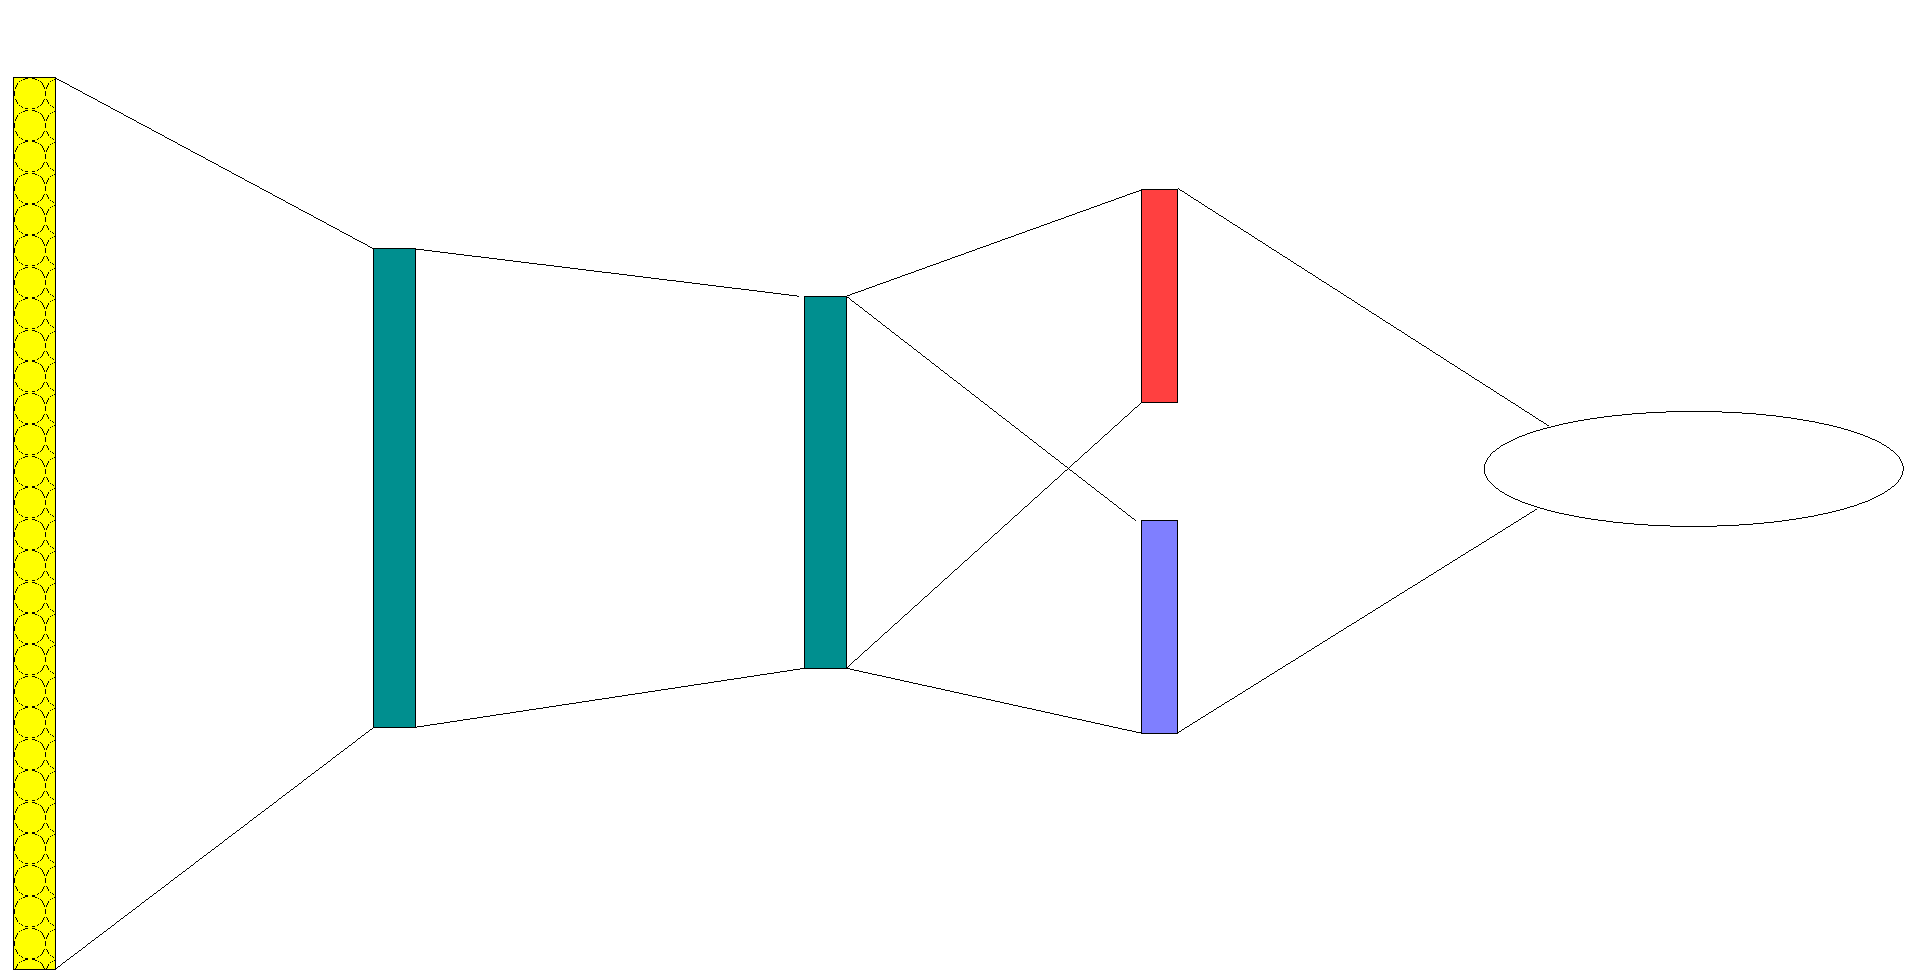
\includegraphics{figures/archi.pdf}%
\end{picture}%
\setlength{\unitlength}{4144sp}%
%
\begingroup\makeatletter\ifx\SetFigFont\undefined%
\gdef\SetFigFont#1#2#3#4#5{%
  \reset@font\fontsize{#1}{#2pt}%
  \fontfamily{#3}\fontseries{#4}\fontshape{#5}%
  \selectfont}%
\fi\endgroup%
\begin{picture}(14512,7383)(3361,-7948)
\put(6121,-2131){\makebox(0,0)[lb]{\smash{{\SetFigFont{29}{34.8}{\rmdefault}{\mddefault}{\updefault}$n_1^h$}}}}
\put(3376,-916){\makebox(0,0)[lb]{\smash{{\SetFigFont{29}{34.8}{\rmdefault}{\mddefault}{\updefault}$n^v$}}}}
\put(7066,-6676){\makebox(0,0)[lb]{\smash{{\SetFigFont{20}{24.0}{\rmdefault}{\mddefault}{\updefault}hidden layers}}}}
\put(10441,-5236){\makebox(0,0)[lb]{\smash{{\SetFigFont{20}{24.0}{\rmdefault}{\mddefault}{\updefault}soft max}}}}
\put(10036,-3076){\makebox(0,0)[lb]{\smash{{\SetFigFont{20}{24.0}{\rmdefault}{\mddefault}{\updefault}fully connected}}}}
\put(7021,-4246){\makebox(0,0)[lb]{\smash{{\SetFigFont{20}{24.0}{\rmdefault}{\mddefault}{\updefault}fully connected}}}}
\put(11926,-1321){\makebox(0,0)[lb]{\smash{{\SetFigFont{29}{34.8}{\rmdefault}{\mddefault}{\updefault}$2n$}}}}
\put(9406,-2131){\makebox(0,0)[lb]{\smash{{\SetFigFont{29}{34.8}{\rmdefault}{\mddefault}{\updefault}$n_2^h$}}}}
\put(3421,-4471){\makebox(0,0)[lb]{\smash{{\SetFigFont{50}{60.0}{\rmdefault}{\mddefault}{\updefault}$X$}}}}
\put(15166,-4246){\makebox(0,0)[lb]{\smash{{\SetFigFont{29}{34.8}{\rmdefault}{\mddefault}{\updefault}$(\hat y(x),\hat I(x))$}}}}
\put(12061,-2941){\makebox(0,0)[lb]{\smash{{\SetFigFont{50}{60.0}{\rmdefault}{\mddefault}{\updefault}$\hat {\bf y}$}}}}
\put(12061,-5506){\makebox(0,0)[lb]{\smash{{\SetFigFont{50}{60.0}{\rmdefault}{\mddefault}{\updefault}$\hat {\bf p}$}}}}
\end{picture}%
}}
\caption{\label{fig:archi} Architecture of the neural network specified by the number of units 
$(n^v,n_1^h,n_2^h,2\vert T\vert)$ in each layer.}
\label{fig:NN}
\end{figure}

\section{Experimental Setting}\label{sec:pdtExp}

\begin{table}[ht]
  \caption{
    Synthetic and Real-World Problems. 
    For the solar wind problem, training and test data sizes represent one cross validation fold}
  \label{tab:exp_data_info}
  \centering
  \begin{tabular}{ r c c c c}
  \hline
  Problem &  \# train & \# test & $d$ & $|T|$ \\
  \hline
  \textbf{I} & $10,000$ & $2,000$  & $10$ & $15$\\
  \textbf{II} & $10,000$ & $2,000$ & $10$ & $20$\\
  \textbf{III} & $10,000$ & $2,000$ & $10$ & $20$\\
  \textbf{IV} & $10,000$ & $2,000$ & $10$ & $20$\\
  \textbf{Solar Wind} & $77,367$ & $648$ & $374$ & $12$\\
  \hline
  \end{tabular}
\end{table}

%Proofs of concept for the  \XX\ algorithm are obtained using synthetic problems as well as our real-world %motivating application, the prediction of the solar wind (\cref{sec:intro}). 
The goal of the experiments is twofold. Firstly, the \XX\ predictive performance is assessed by 
considering 
%
\begin{enumerate*} 
  \item the RMSE of the predicted effect series $\hat y_t$, computed from Eq. (\ref{prop:opred})  
  \item the accuracy of the time lag prediction 
\end{enumerate*}. 
%
The latter performance indicator is measured and compared to the ground truth using synthetic 
problems, detailed below: although time lag relationships do exist in real world data sets 
\citep{doi:10.1002/jgra.50429,ZHOU2006195}, we are not aware of datasets with time lag 
relationships explicitly annotated. The former performance indicator is comparatively assessed 
using the naive baseline, the regression model computed by assuming a fixed time lag set to 
$\frac{\Delta t_{min} + \Delta t_{max}}{2}$. The Pearson correlation of between $y_t$ and 
the predicted $\hat y_t$ series is also considered as overall performance indicator of the prediction.

The second goal of experiments is to determine how informative are the key statistical quantities 
$\sigma_0$ and $C_1$ (\cref{sec:stability}), and whether they can effectively be used as 
measures of confidence about the prediction results. Table \ref{tab:exp_data_info} summarises the 
dimensions of the synthetic and real problems used as proofs of concept for the \XX\ validation. 

\paragraph{Synthetic Problems.}
Four synthetic problems of increasing difficulty are generated using 
\emph{Stochastic Langevin Dynamics}. In all problems, the cause signal 
$\mathbf{x}_t \in \mathbb{R}^{10}$ and the effect signal $y_t$ are generated as follows 
(with $\eta = 0.02, s^2 = 0.7$): 
\begin{align}
 \mathbf{x}_{t+1} &= (1 - \eta) \mathbf{x}_t + \mathcal{N}(0, s^2) \label{eq:data}\\
 v_t &= k ||\mathbf{x}_t||^2 + c\\
 y_{t+g(\mathbf{x}_t)} &= f(v_t), \label{eq:outputs}
\end{align} 
with time-lag mapping $g(\mathbf{x}_t)$ ranges in a time interval with width $20$ 
(except for problem I where $|T| = 15$). The complexity of the synthetic 
problems is governed by the amplitude and time-lag functions $f$ and $g$, as 
shown in the table below.\\

\centerline{  
  \resizebox{\textwidth}{!}{
    \begin{tabular}{ l c l l }
      \hline
      Problem &  $f(v_t)$ & $g(\mathbf{x}_t)$ & Other\\
      \hline
      \textbf{I} & $v_t$ & $5$ & $k = 10,c=0$\\
      \textbf{II} & $v_t$ & $100/v_t$ & $k = 1, c = 10$\\
      \textbf{III} & $\sqrt{v^2_{t} + 2ad}$ & $(\sqrt{v_t^2 + 2ad} - v)/a$ & $k = 5, a = 5, d = 1000, c = 100$\\
      \textbf{IV} & $v_t$ & $g(\mathbf{x}_t) = \exp\left(v_t\right)/\left(1 + \exp(v_t/20)\right)$ & $k = 10, c = 40$\\
      \hline
      \end{tabular}
  }
}

\paragraph{Solar Wind Speed Prediction}\label{sec:solarwind}
As said in \cref{sec:motivationsolarwind}, the task of predicting solar wind speed from 
heliospheric data not only has scientific significance; it is also challenging due to the distance 
between the Sun and the Earth and the non-stationary propagation time of the solar plasma through 
the interplanetary medium. 

The inputs $\mathbf{x}_t$ are compiled from two sources, synoptic Carrington maps of the photospheric 
magnetic field taken from the \emph{Global Oscillation Network Group} (GONG) and solar activity 
proxies taken from the OMNI data set\footnote{\url{https://omniweb.gsfc.nasa.gov}}. Specifically, 
$\mathbf{x}_t$ is a vector consisting of the components outlined in \cref{table:dtlrInputs}.

For each input pattern, time lagged solar wind data is extracted corresponding to minimum and 
maximum time delays of two and five days respectively. For computational convenience, each three 
day time window is pre-processed by computing sliding six hour medians yielding $|T| = 12$ time 
slots\footnote{Before computing the cross-validation performance, the predictions are mapped back to 
hourly resolution using interpolation}. Before training, the solar wind data was 
mapped into standardized Gaussian space by applying a quantile-quantile followed 
by the inverse probit mapping.
%
\begin{table}[ht]
    \centering
    \begin{tabular}{l l l p{0.4\textwidth}}
        \hline
        \textbf{Quantity} & \textbf{Source} & \textbf{Domain} & \textbf{Notes}\\
        \hline
        \vspace{5pt}
          $\log \mathbf{f}_S$ & 
          GONG & 
          $\mathbb{R}^{180}$ & 
          $\mathbf{f}_S$ or FTE is computed from the outputs of the CSSS model.\\
          $\mathbf{B}_{cp}$ & 
          GONG & 
          $\mathbb{R}^{180}$  & 
          The radial magnetic field strength on the solar cusp surface is the primary output computed by the CSSS model.\\
          $\mathbf{v}_{27}$ & 
          OMNI & 
          $\mathbb{R}^{\rvert T \rvert}$ & 
          $\mathbf{v}_{27}$ is the solar wind speed recorded $27$ days prior, one for each value of the forward time window. \\
          $\mathrm{SSN}$ & OMNI & $\mathbb{R}^{+}$ & The sun spot number measures the number of visible sun spots on the solar disk. \\
          $\mathrm{F}10.7$ & OMNI & $\mathbb{R}^{+}$ & $\mathrm{F}10.7$ is the measured solar radio flux. \\
        \hline
    \end{tabular}
    \caption{Inputs used in the DTLR solar wind forecast model.}
    \label{table:dtlrInputs}
\end{table}

\XX\ is validated using a $9$ fold cross-validation, where the test data consists of one 
(continuous) Carrington rotation (see \cref{table:dtlrsplits}). The performance on Carrington 
rotation $2077$ (first fold in \cref{table:dtlrsplits}) is compared with the state of the art 
\citep{Riley2011} in \cref{tab:results_reiss}, while the overall cross-validation performance 
is compared with a fixed time lag baseline which uses the same inputs as the DTLR model 
(\cref{table:dtlrInputs}) and has the same architecture until the penultimate layer 
(\cref{fig:archi}). For Carrington rotations $2077$ and $2184$, the hourly solar wind 
time series reconstructions are shown in \cref{fig:problemsw_ts1,fig:problemsw_ts2} respectively. 

%
\begin{table}[ht]
  \centering
  \caption{Cross validation splits used to evaluate \ \XX \ on the solar wind forecasting task}
  \label{table:dtlrsplits}
  \resizebox{\textwidth}{!}{
    \begin{tabular}{llll}
      \hline
      \textbf{Split Id} & \textbf{Carrington Rotation} & \textbf{Start} & \textbf{End}\\ \hline
      $1$ & $2077$ & 2008/11/20 07:00:04 & 2008/12/17 14:38:34  \\
      $2$ & $2090$ & 2009/11/09 20:33:43 & 2009/12/07 04:03:59  \\
      $3$ & $2104$ & 2010/11/26 17:32:44 & 2010/12/24 01:15:56  \\
      $4$ & $2117$ & 2011/11/16 07:04:41 & 2011/12/13 14:39:28  \\
      $5$ & $2130$ & 2012/11/04 20:39:43 & 2012/12/02 04:06:23  \\
      $6$ & $2143$ & 2013/10/25 10:17:52 & 2013/11/21 17:36:35  \\
      $7$ & $2157$ & 2014/11/11 07:09:56 & 2014/12/08 14:41:02  \\
      $8$ & $2171$ & 2015/11/28 04:09:27 & 2015/12/25 11:53:33  \\
      $9$ & $2184$ & 2016/11/16 17:41:04 & 2016/12/14 01:16:43  \\
      \hline
      \end{tabular}
  }
  \end{table}
%


\section{Empirical validation}\label{sec:proofconcept}

\begin{figure*}
  \centering

  \begin{subfigure}[b]{0.4\textwidth}
    \centering
    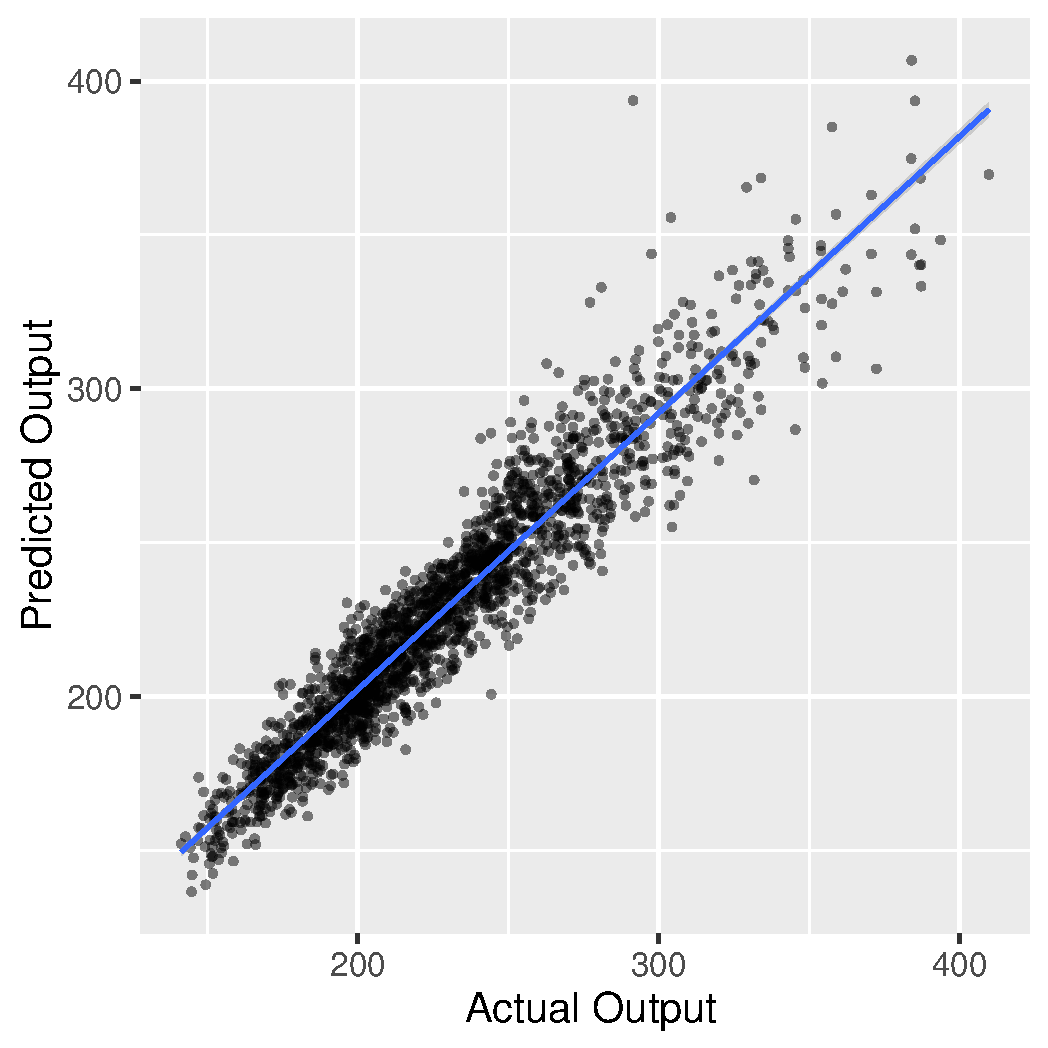
\includegraphics[width=\textwidth]{figures/exp2_scatter_v_test}
    \caption{ \textbf{Problem II}, Goodness of fit, Output $y(x)$}
    \label{fig:problem2_fitv}
  \end{subfigure}
  \hfill
  \begin{subfigure}[b]{0.4\textwidth}
    \centering
    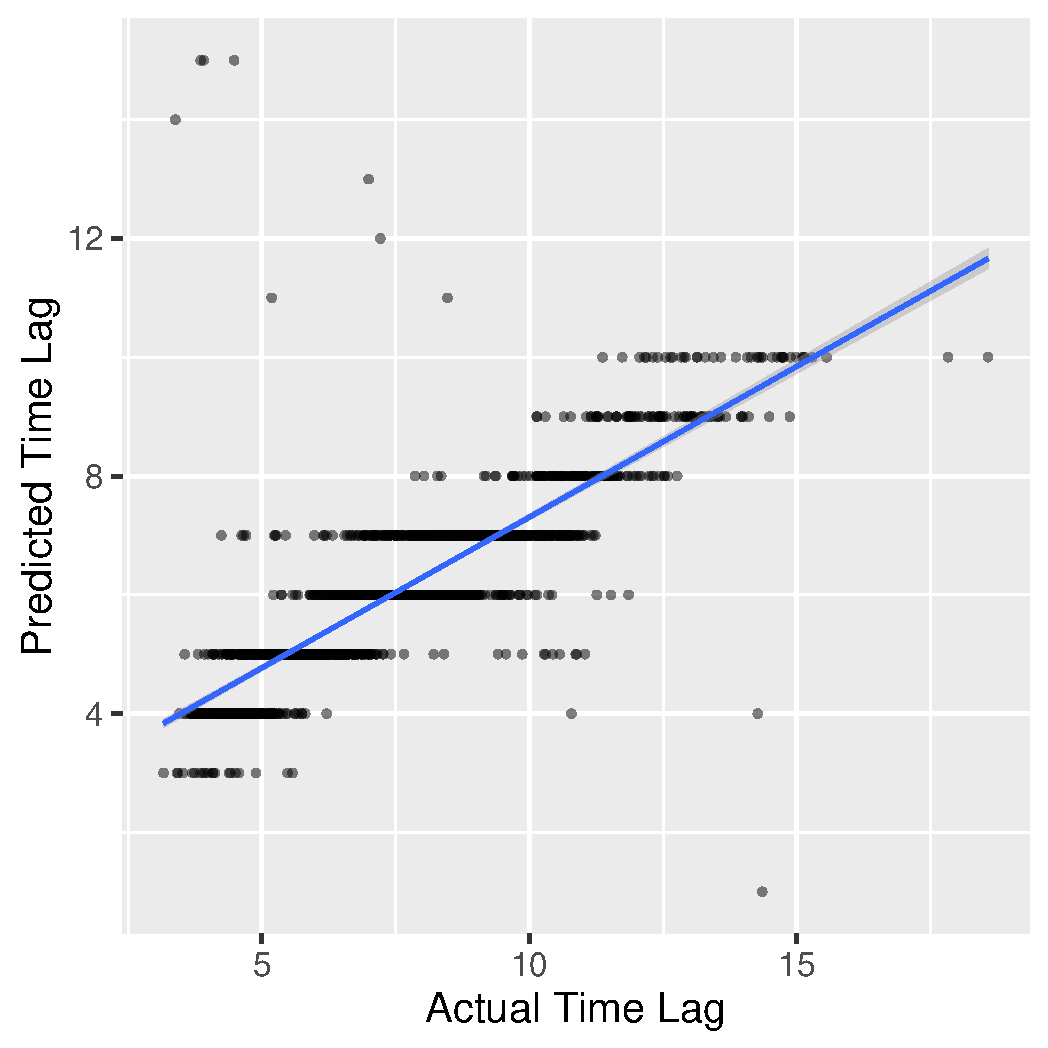
\includegraphics[width=\textwidth]{figures/exp2_scatter_t_test}
    \caption{ \textbf{Problem II}, Goodness of fit, Time lag $\tau(t)$ }
    \label{fig:problem2_fitt}
  \end{subfigure}
  
  \vskip\baselineskip
  
  \begin{subfigure}[b]{0.4\textwidth}
    \centering
    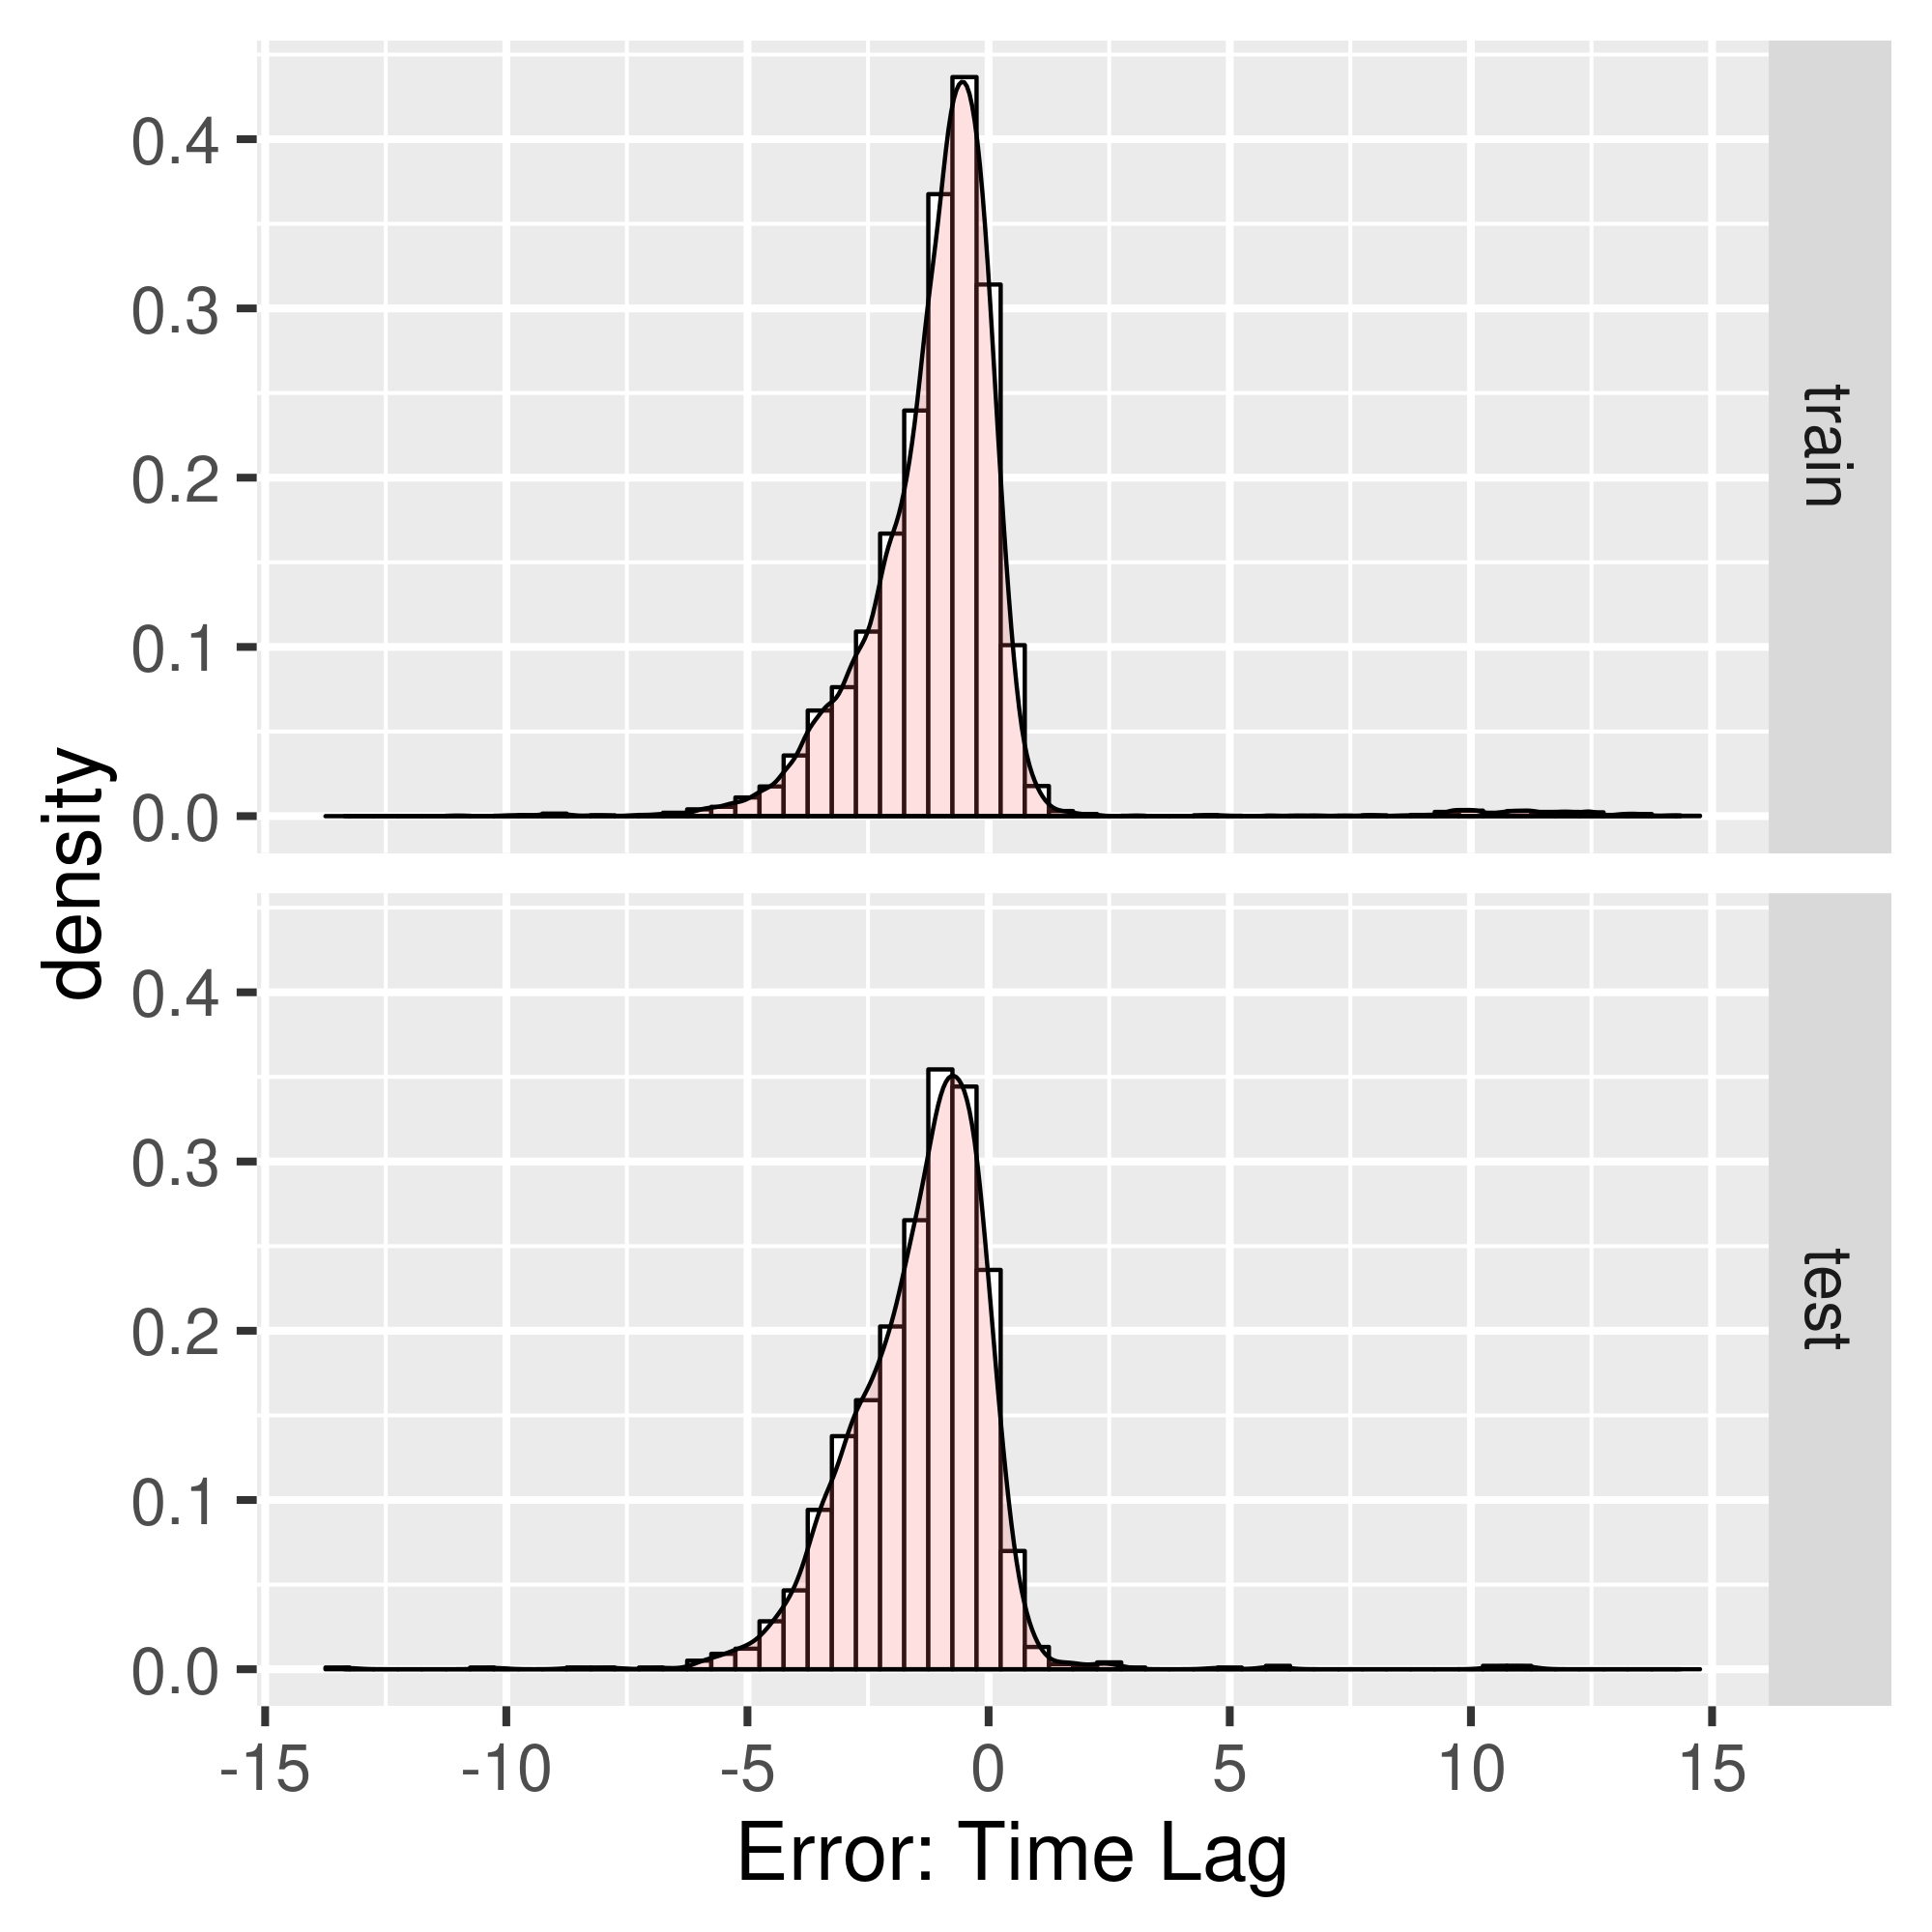
\includegraphics[width=\textwidth]{figures/exp2_hist_errors_timelag}
    \caption{ \textbf{Problem II}, Error of time lag prediction} 
    \label{fig:problem2_error}
  \end{subfigure}
  \hfill
  \begin{subfigure}[b]{0.4\textwidth}
    \centering
    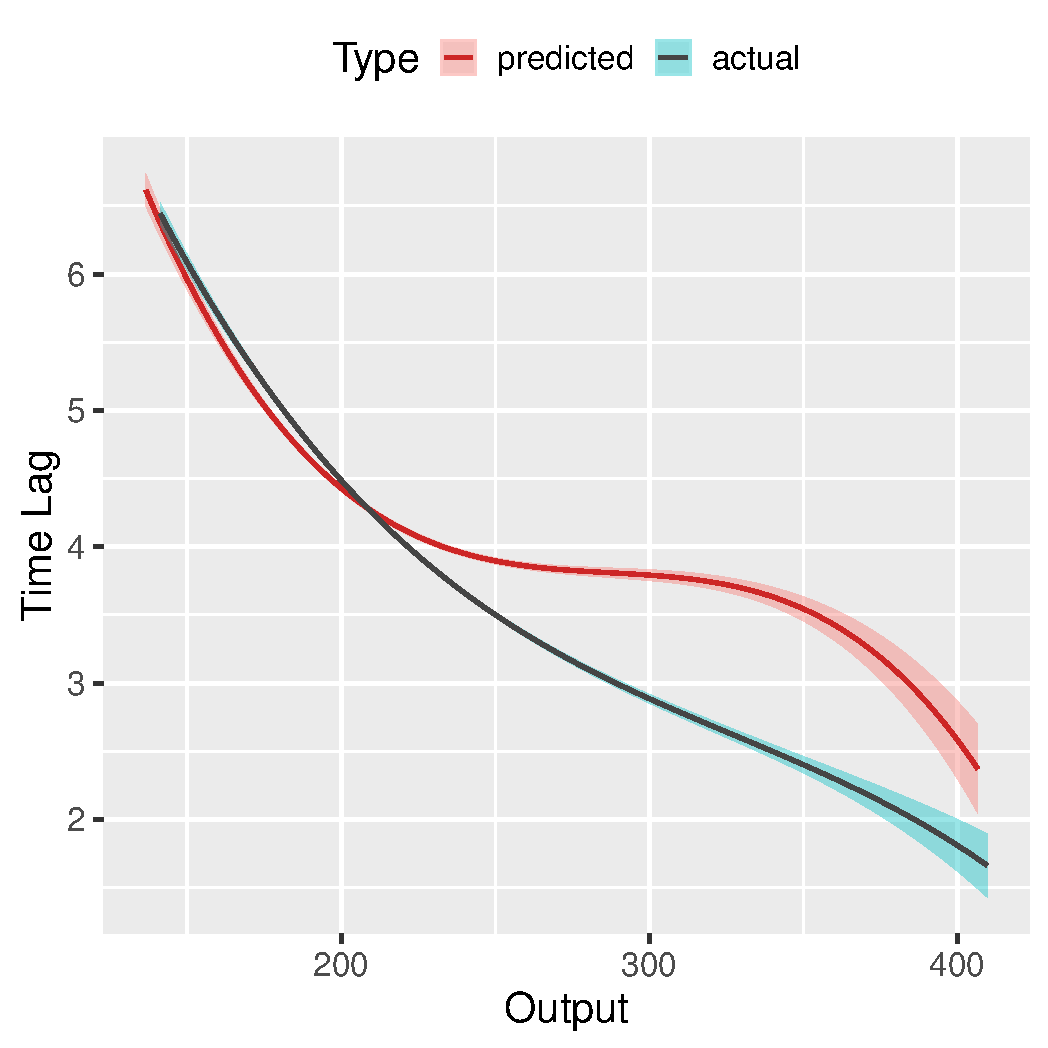
\includegraphics[width=\textwidth]{figures/exp2_predictive_curves}
    \caption{ \textbf{Problem II}, Output vs Time Lag Relationship} 
    \label{fig:problem2_curves}
  \end{subfigure}

  %\vskip\baselineskip
  
  %\begin{subfigure}[b]{0.4\textwidth}
  %  \centering
  %  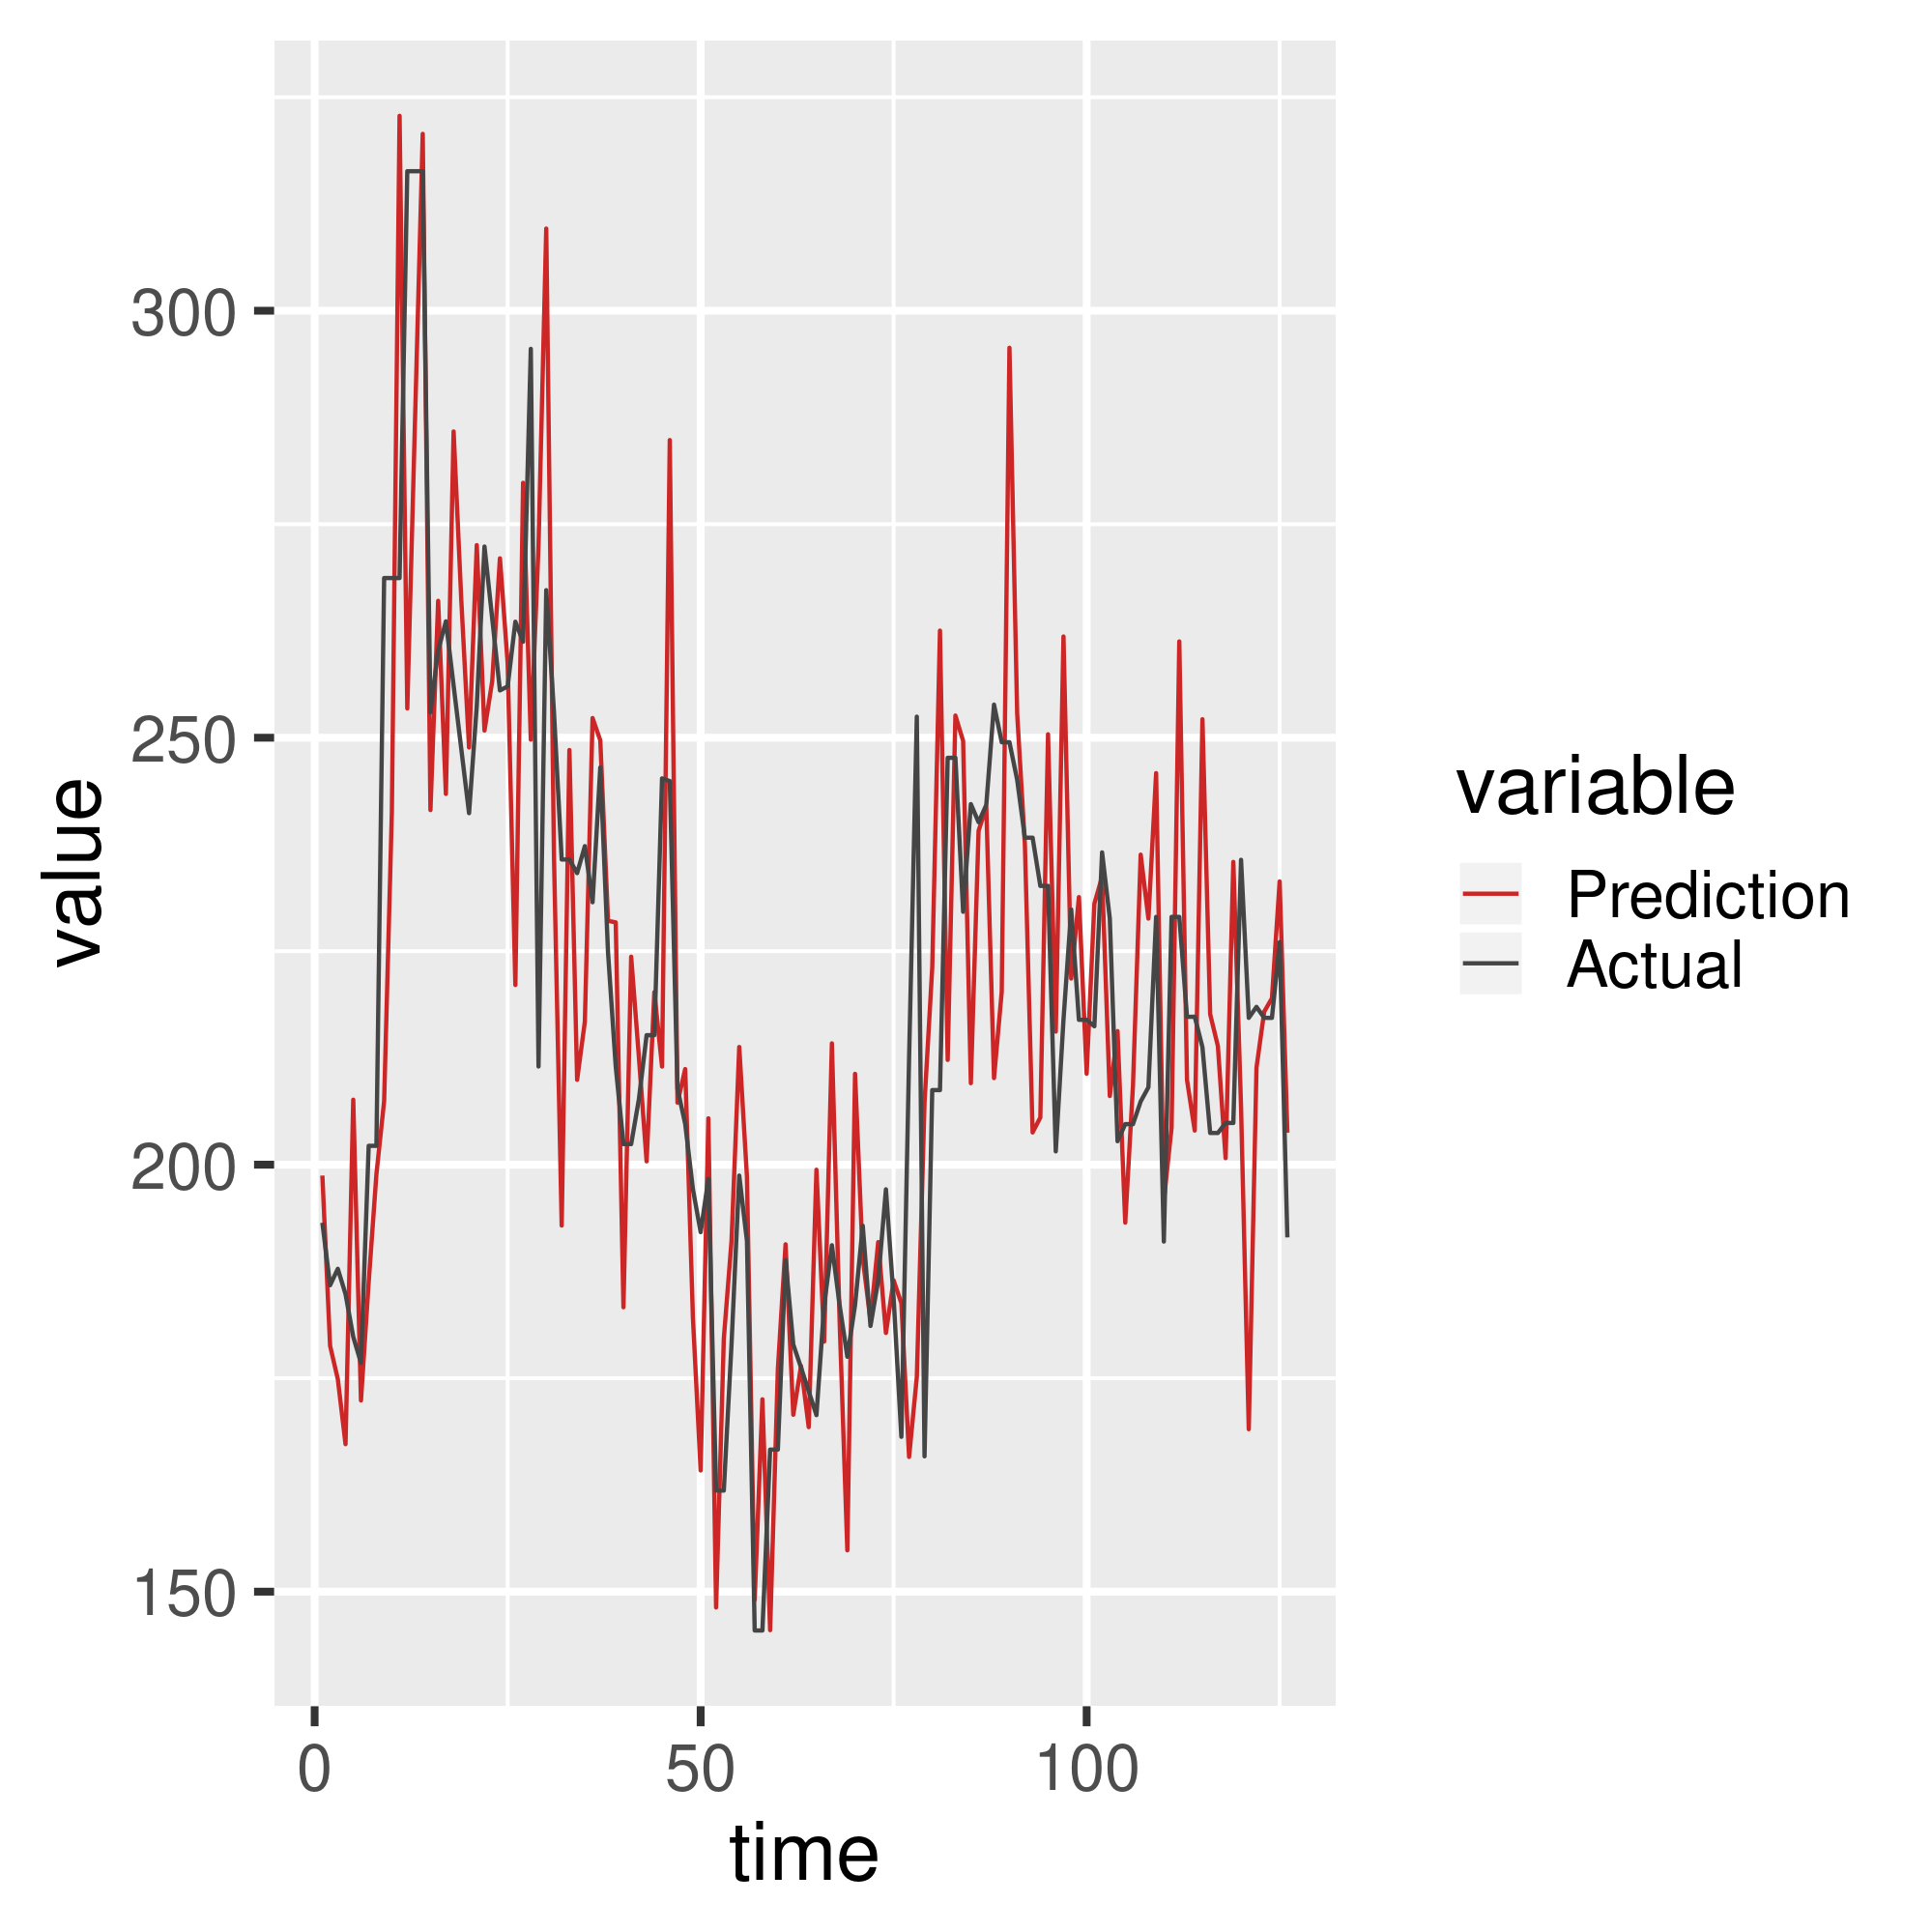
\includegraphics[width=\textwidth]{figures/exp2_timeseries_pred}
  %  \caption{ \textbf{Problem II}, A portion of the test time series reconstructed using the model} 
  %  \label{fig:problem2_timeseries}
  %\end{subfigure}
  %\hfill
  %\begin{subfigure}[b]{0.4\textwidth}
  %  \centering
  %  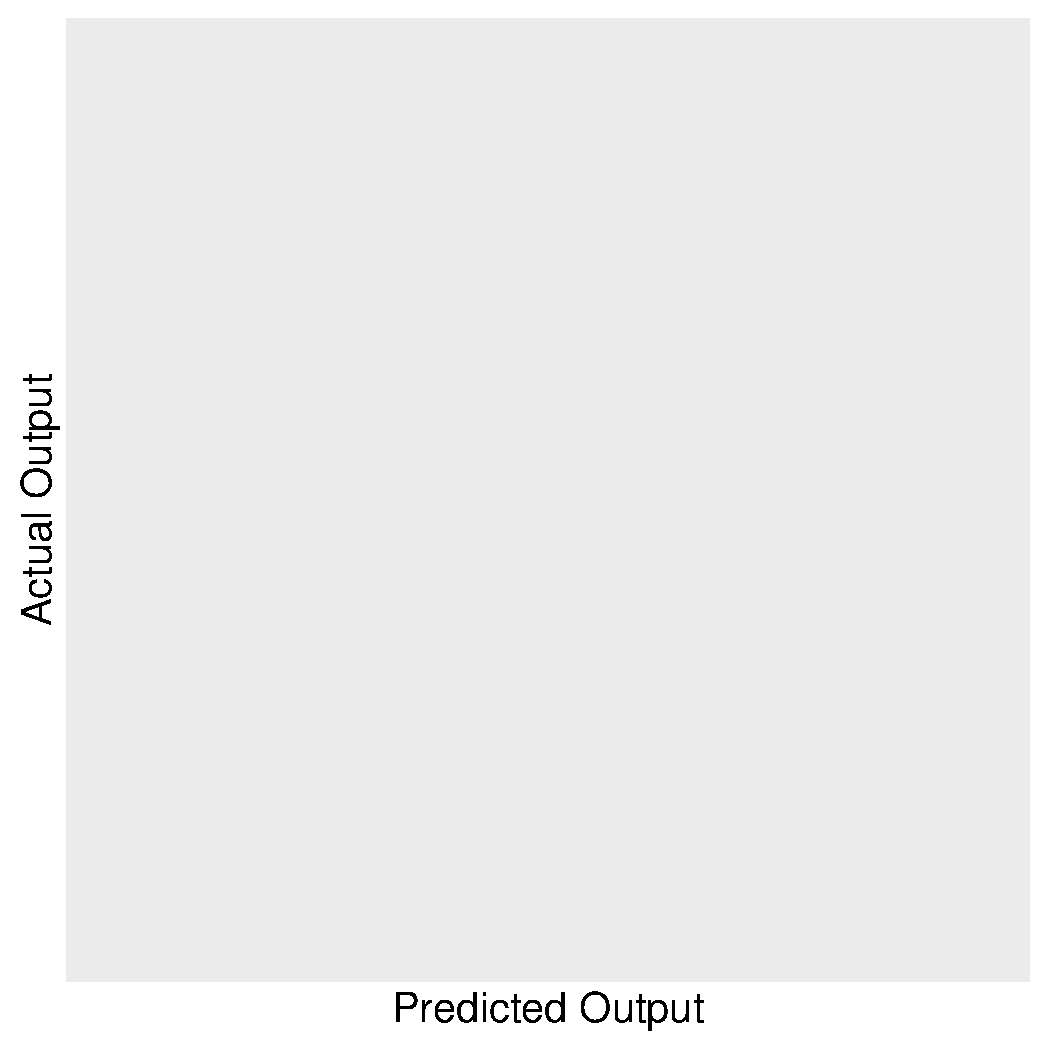
\includegraphics[width=\textwidth]{figures/exp2_lag_error_jus}
  %  \caption{ \textbf{Problem II}, Predicted vs Actual Outputs for the cases with time lag error $\leq -2.5$.} 
  %  \label{fig:problem2_lag_error_jus}
  %\end{subfigure}
  
  \caption{\textbf{Problem II}, Results}
\end{figure*}

\begin{figure*}
  \centering

  \begin{subfigure}[b]{0.4\textwidth}
    \centering
    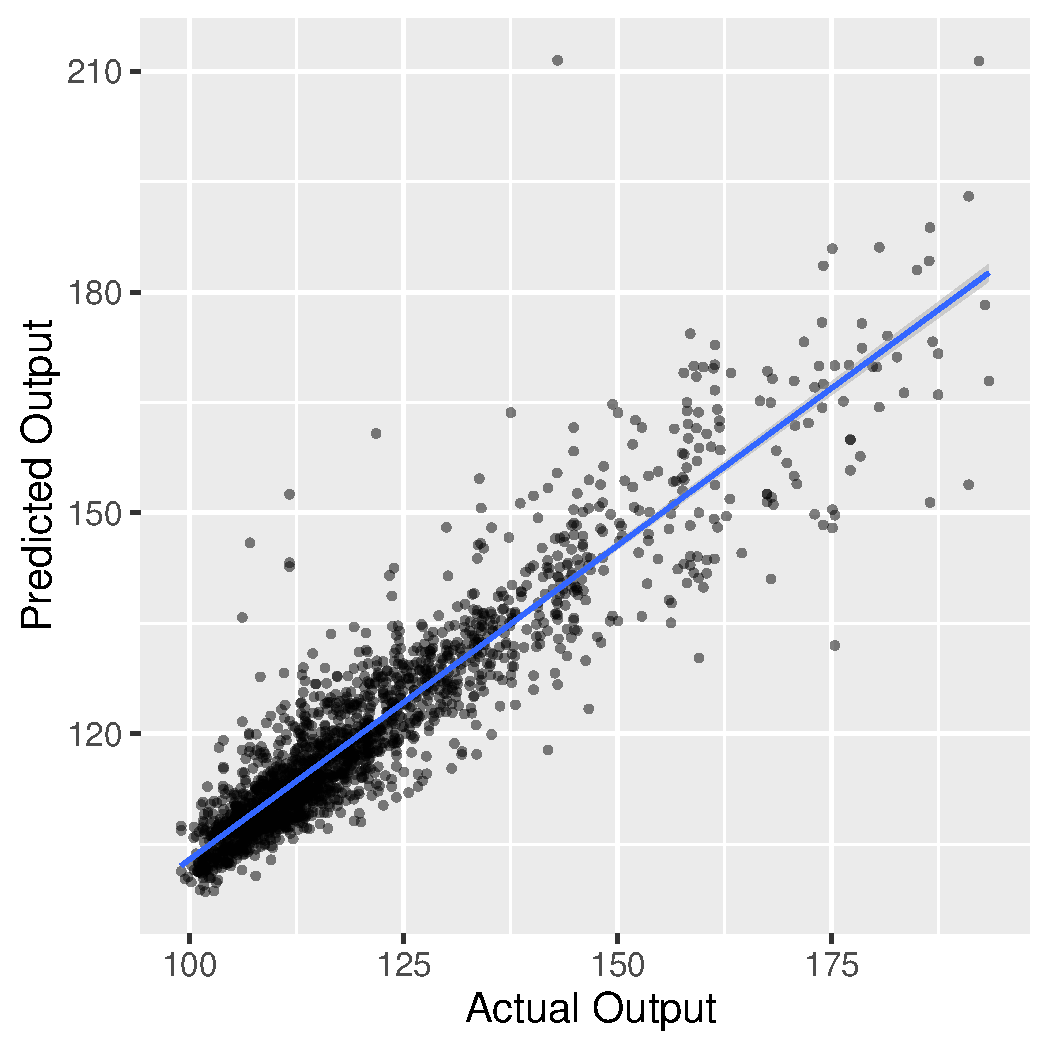
\includegraphics[width=\textwidth]{figures/exp3_scatter_v_test}
    \caption{ \textbf{Problem III}, Goodness of fit, Output $y(x)$}
    \label{fig:problem3_fitv}
  \end{subfigure}
  \hfill
  \begin{subfigure}[b]{0.4\textwidth}
    \centering
    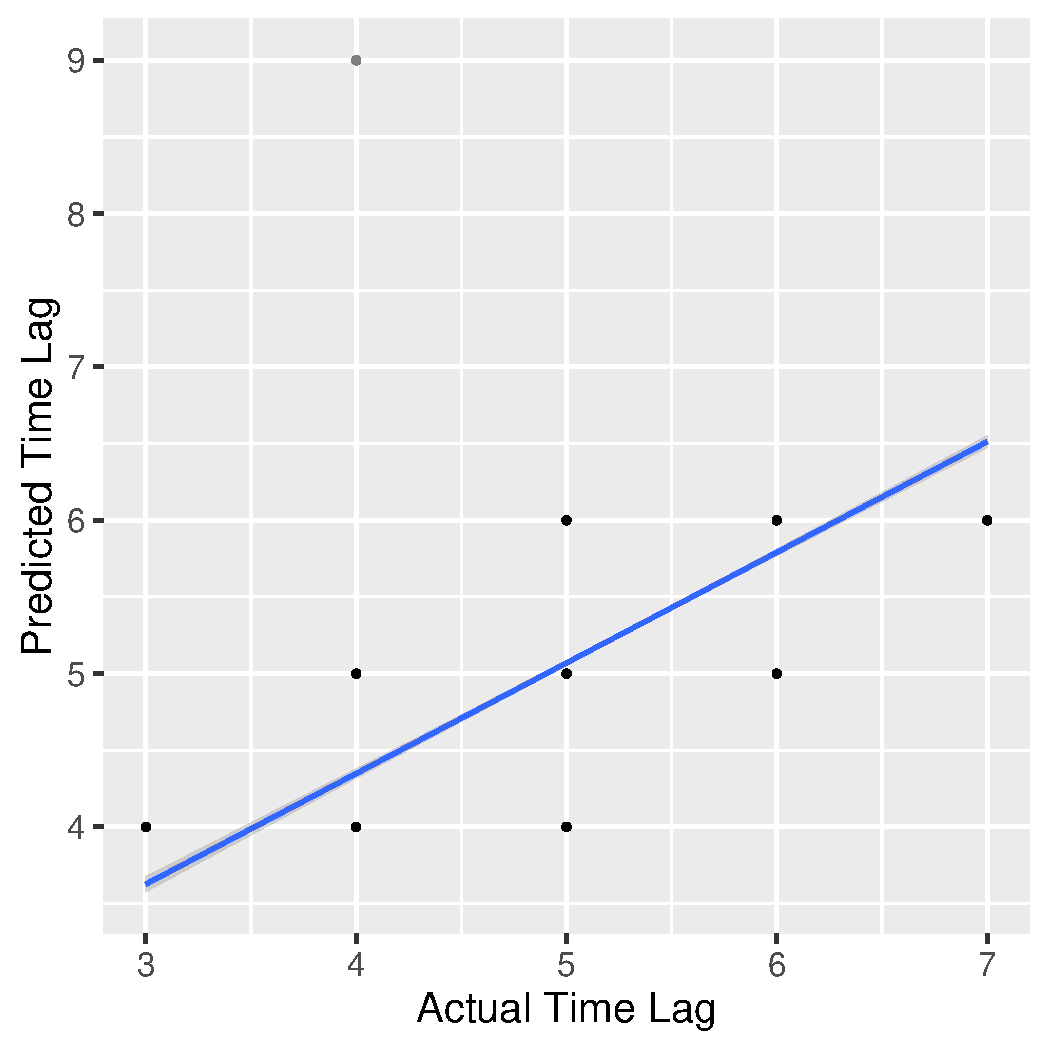
\includegraphics[width=\textwidth]{figures/exp3_scatter_t_test}
    \caption{ \textbf{Problem III}, Goodness of fit, Time lag $\tau(t)$ }
    \label{fig:problem3_fitt}
  \end{subfigure}

  \vskip\baselineskip
  
  \begin{subfigure}[b]{0.4\textwidth}
    \centering
    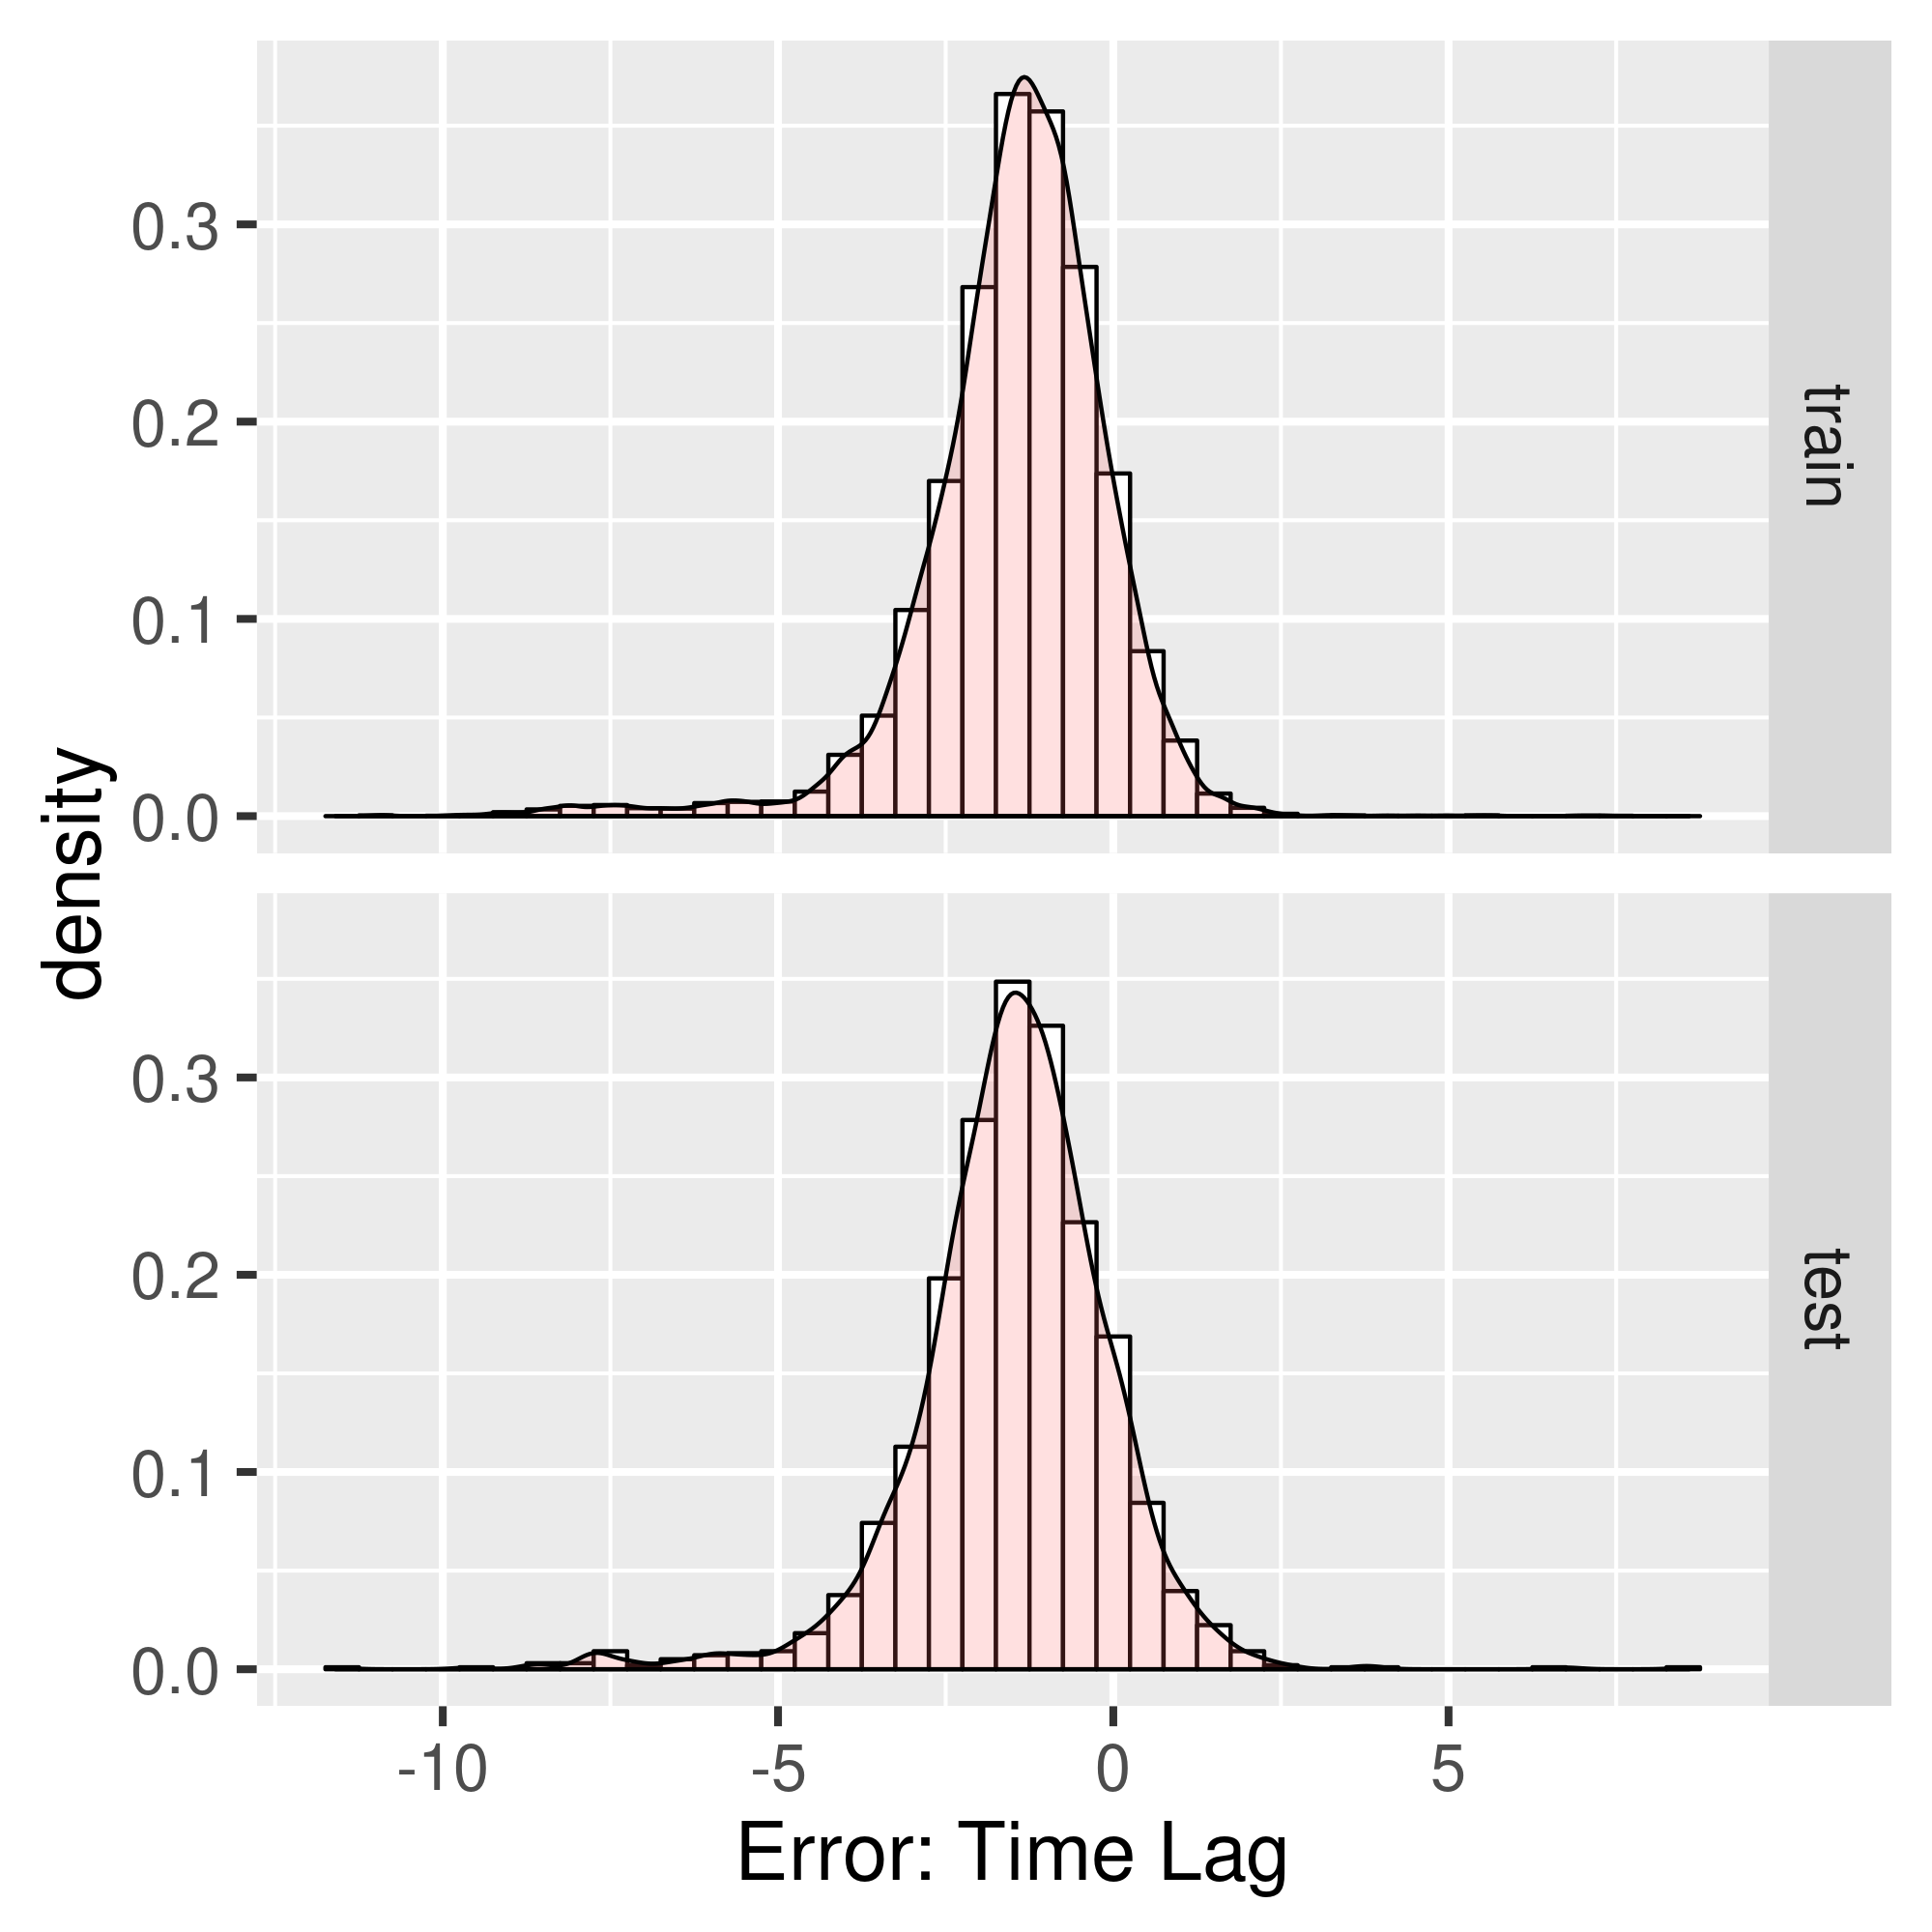
\includegraphics[width=\textwidth]{figures/exp3_hist_errors_timelag}
    \caption{ \textbf{Problem III}, Error of time lag prediction} 
    \label{fig:problem3_error}
  \end{subfigure}
  \hfill
  \begin{subfigure}[b]{0.4\textwidth}
    \centering
    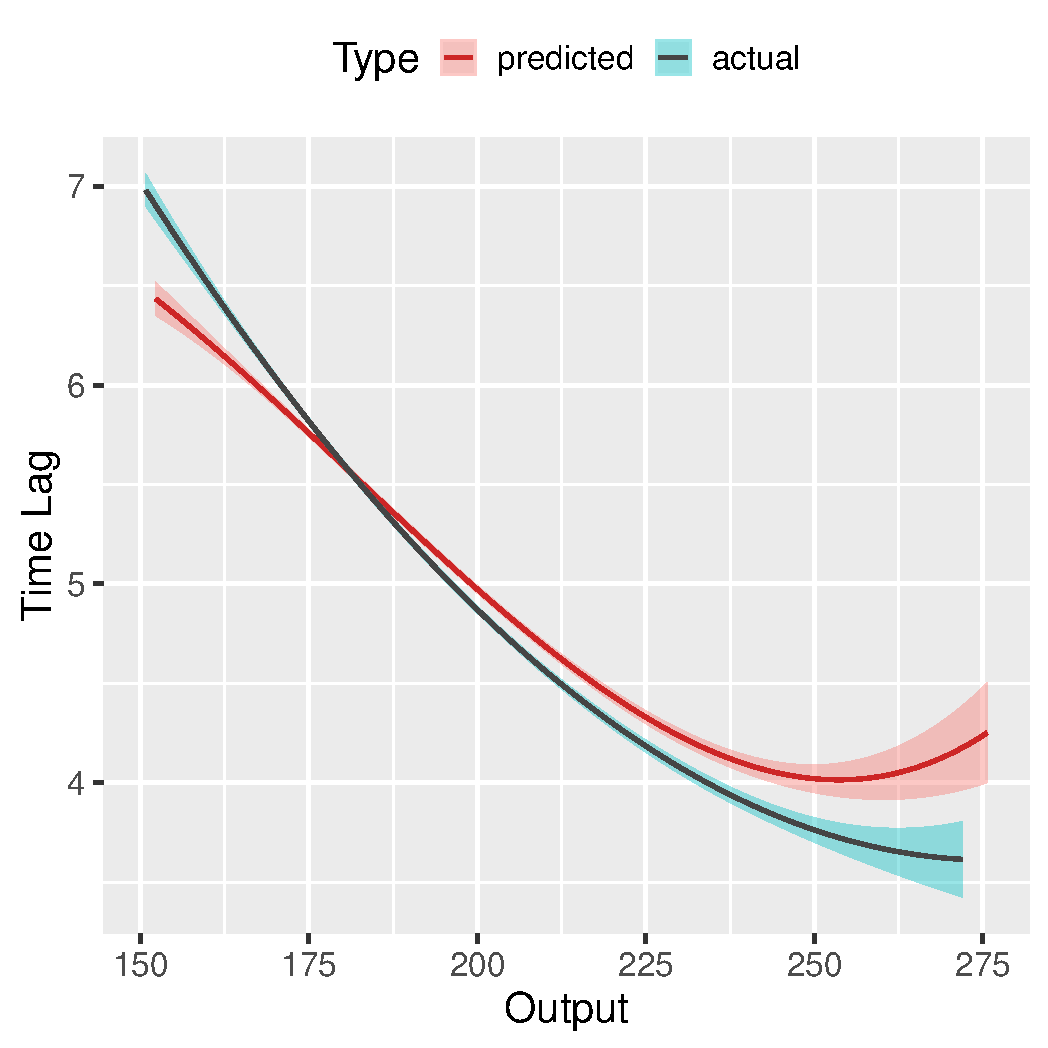
\includegraphics[width=\textwidth]{figures/exp3_predictive_curves}
    \caption{ \textbf{Problem III}, Output vs Time Lag Relationship} 
    \label{fig:problem3_curves}
  \end{subfigure}
  
  %\vskip\baselineskip
  
  %\begin{subfigure}[b]{0.4\textwidth}
  %  \centering
  %  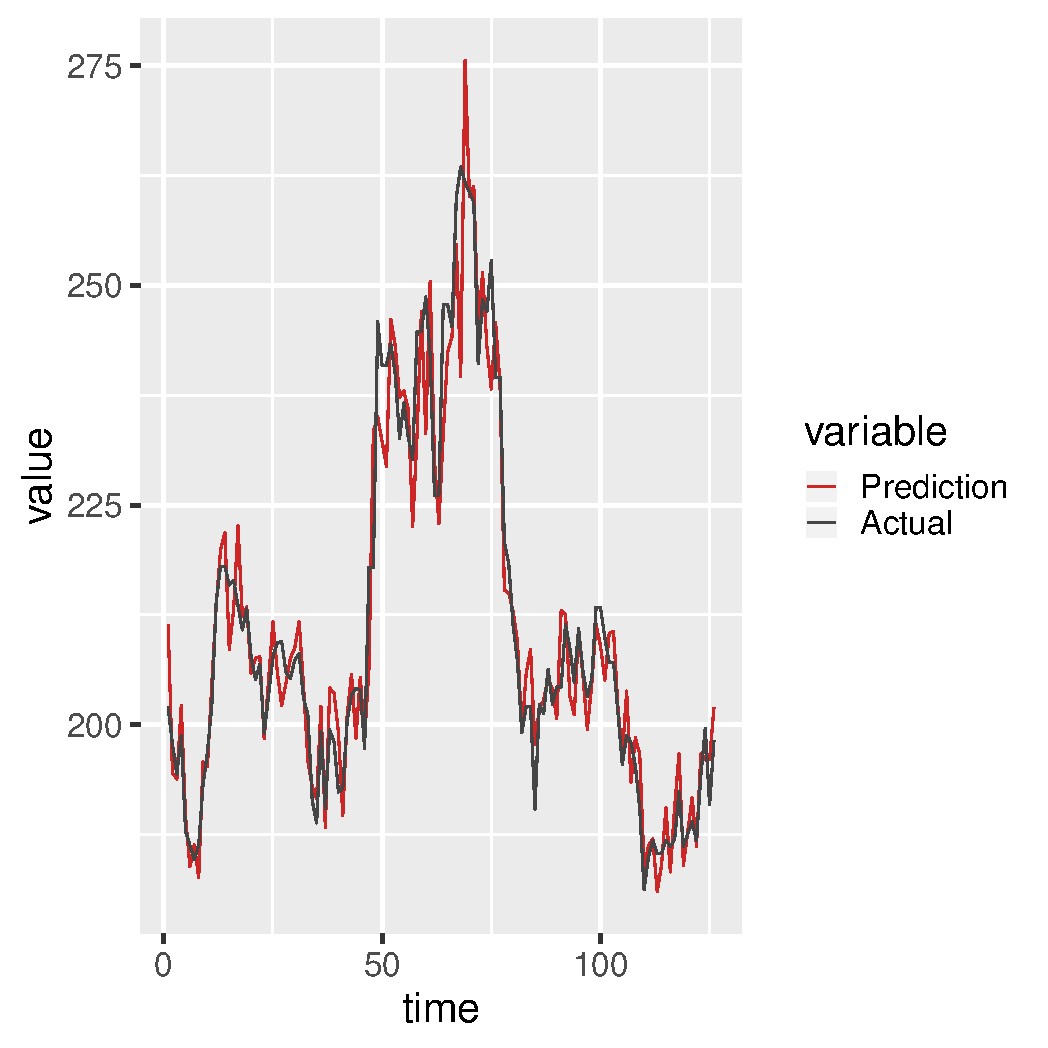
\includegraphics[width=\textwidth]{figures/exp3_timeseries_pred}
  %  \caption{ \textbf{Problem III}, A portion of the test time series reconstructed using the model} 
  %  \label{fig:problem3_timeseries}
  %\end{subfigure}
  %\hfill
  %\begin{subfigure}[b]{0.4\textwidth}
  %  \centering
  %  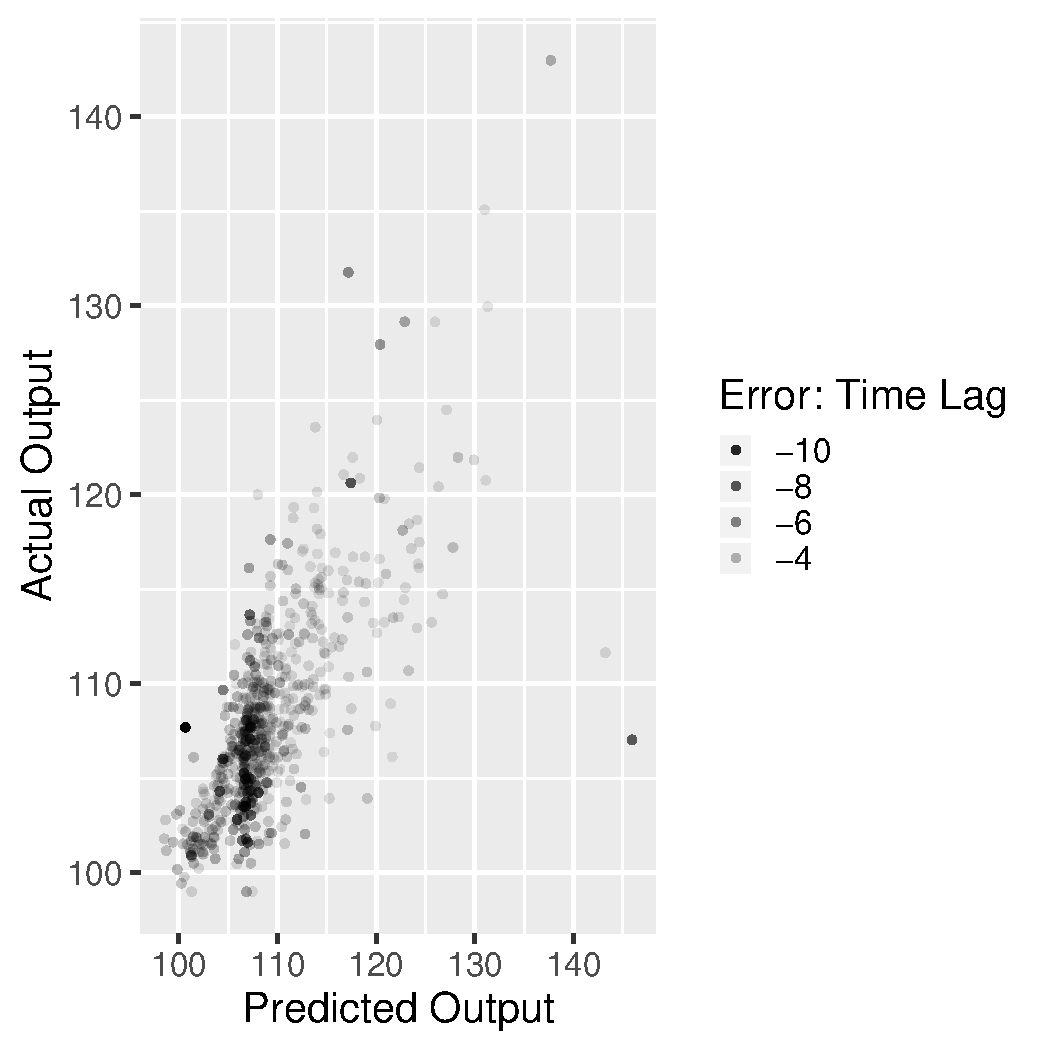
\includegraphics[width=\textwidth]{figures/exp3_lag_error_jus}
  %  \caption{ \textbf{Problem III}, Predicted vs Actual Outputs for the cases with time lag error $\leq -2.5$.} 
  %  \label{fig:problem3_lag_error_jus}
  %\end{subfigure}
  
  \caption{\textbf{Problem III}, Results}
\end{figure*}

\begin{figure*}
  \centering

  \begin{subfigure}[b]{0.4\textwidth}
    \centering
    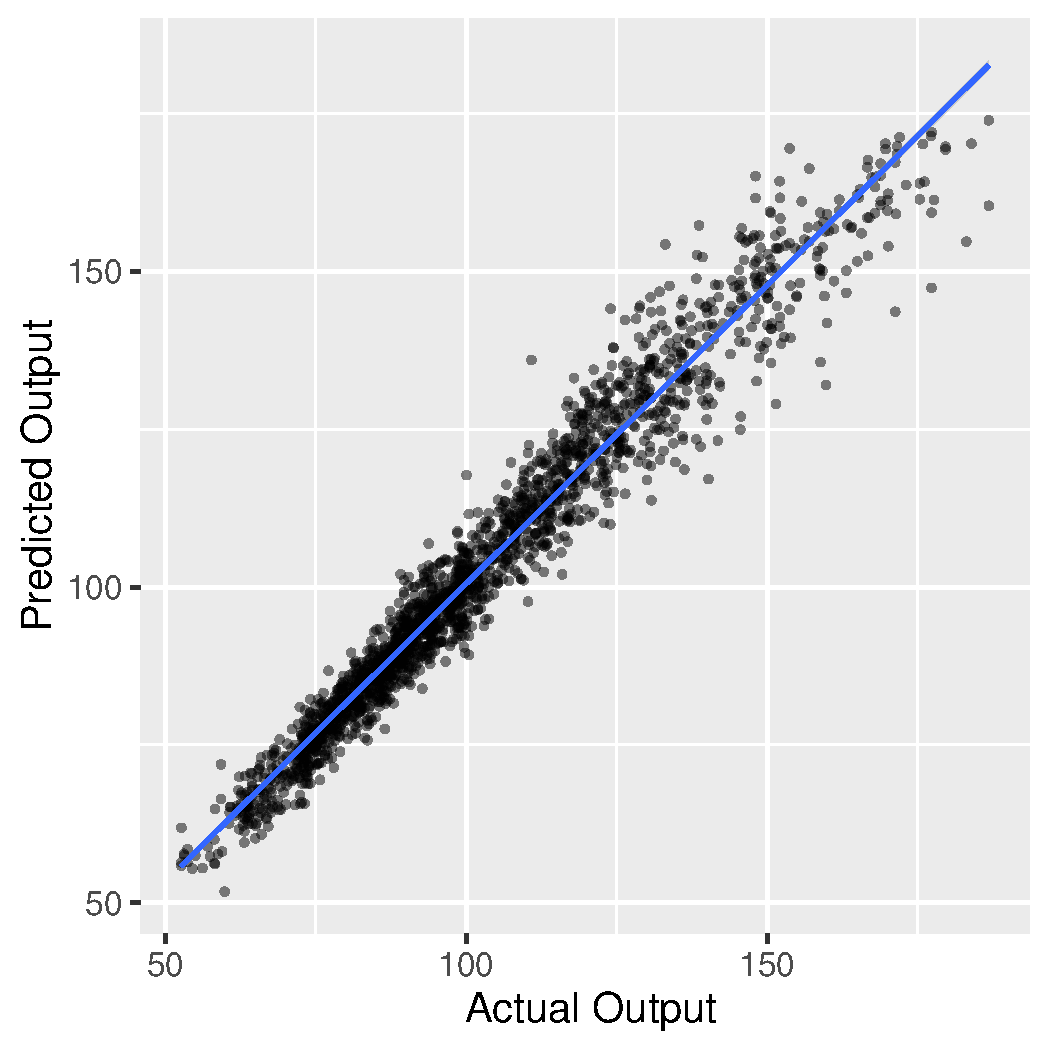
\includegraphics[width=\textwidth]{figures/exp4_scatter_v_test}
    \caption{ \textbf{Problem IV}, Goodness of fit, Output $y(x)$}
    \label{fig:problem4_fitv}
  \end{subfigure}
  \hfill
  \begin{subfigure}[b]{0.4\textwidth}
    \centering
    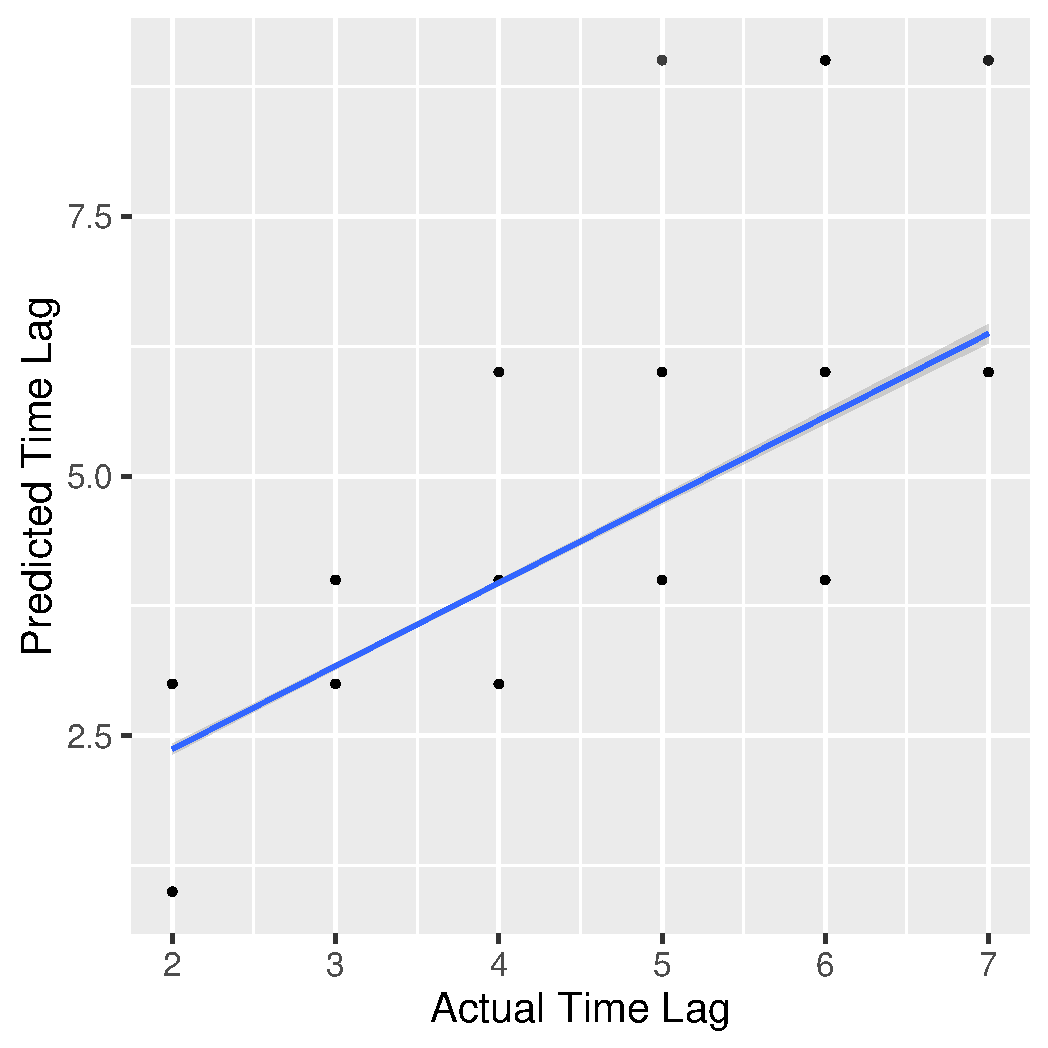
\includegraphics[width=\textwidth]{figures/exp4_scatter_t_test}
    \caption{ \textbf{Problem IV}, Goodness of fit, Time lag $\tau(t)$ }
    \label{fig:problem4_fitt}
  \end{subfigure}
  
  \vskip\baselineskip
  
  \begin{subfigure}[b]{0.4\textwidth}
    \centering
    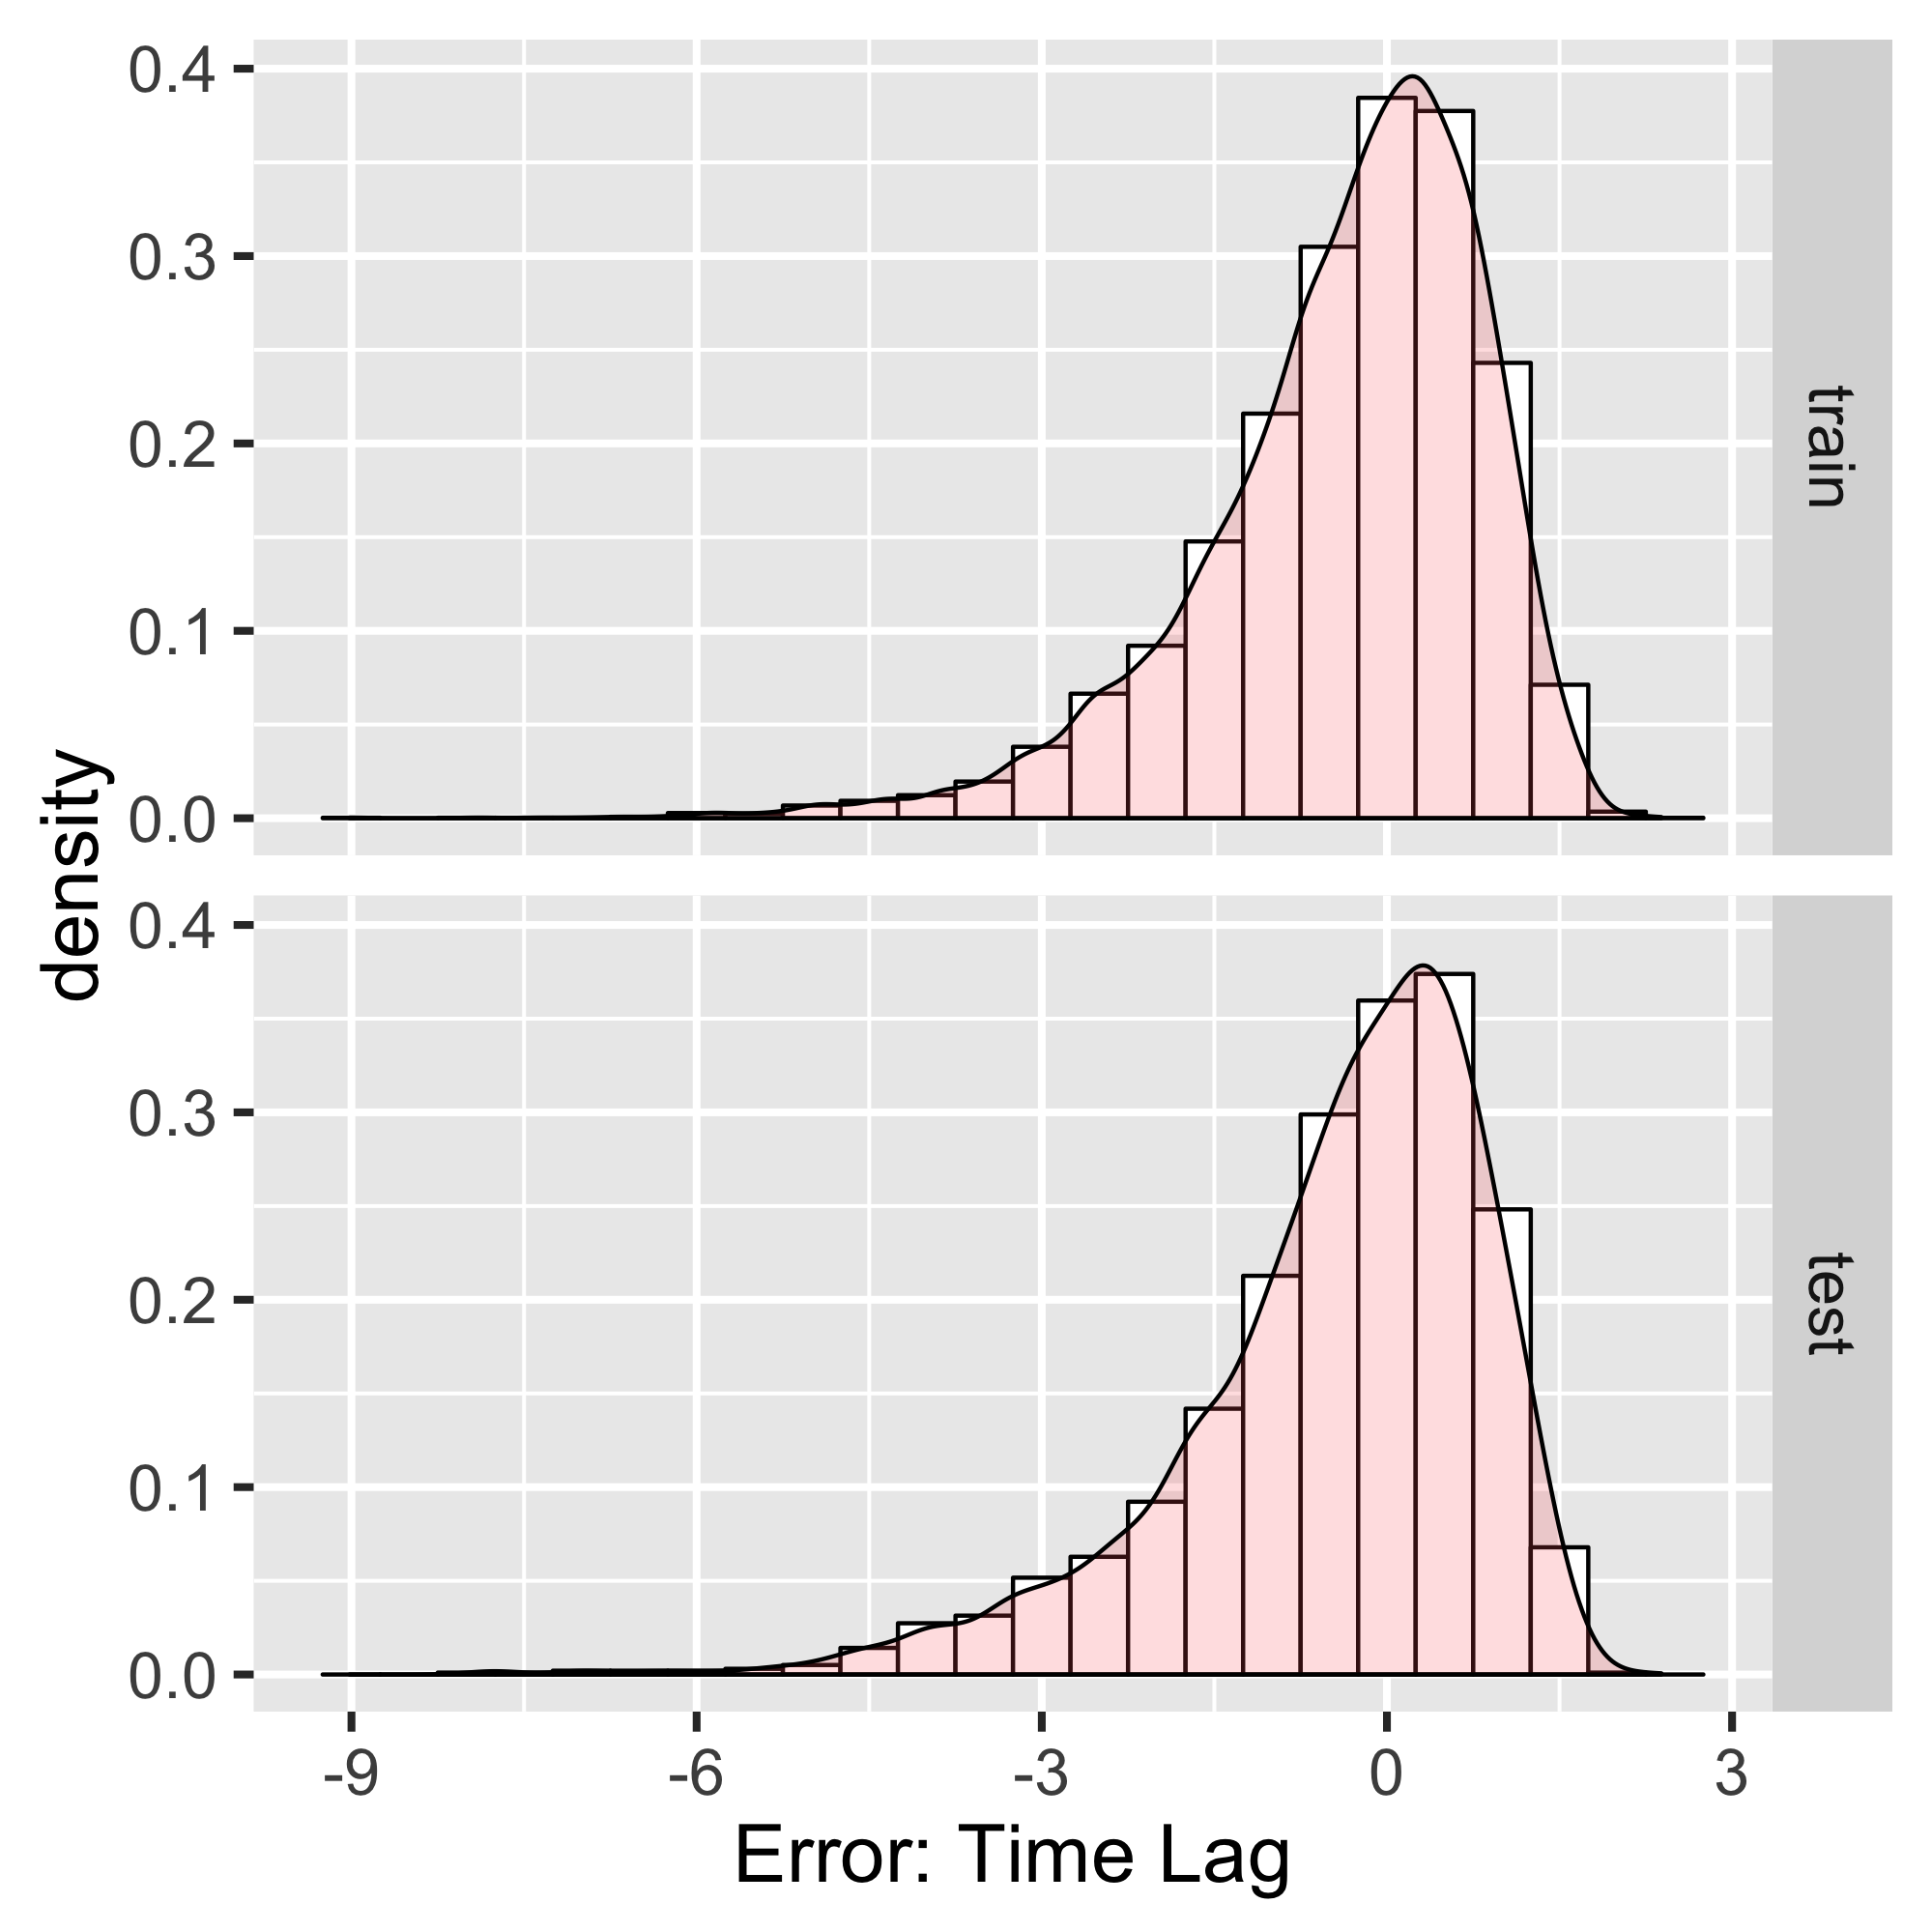
\includegraphics[width=\textwidth]{figures/exp4_hist_errors_timelag}
    \caption{ \textbf{Problem IV}, Error of time lag prediction} 
    \label{fig:problem4_error}
  \end{subfigure}
  \hfill
  \begin{subfigure}[b]{0.4\textwidth}
    \centering
    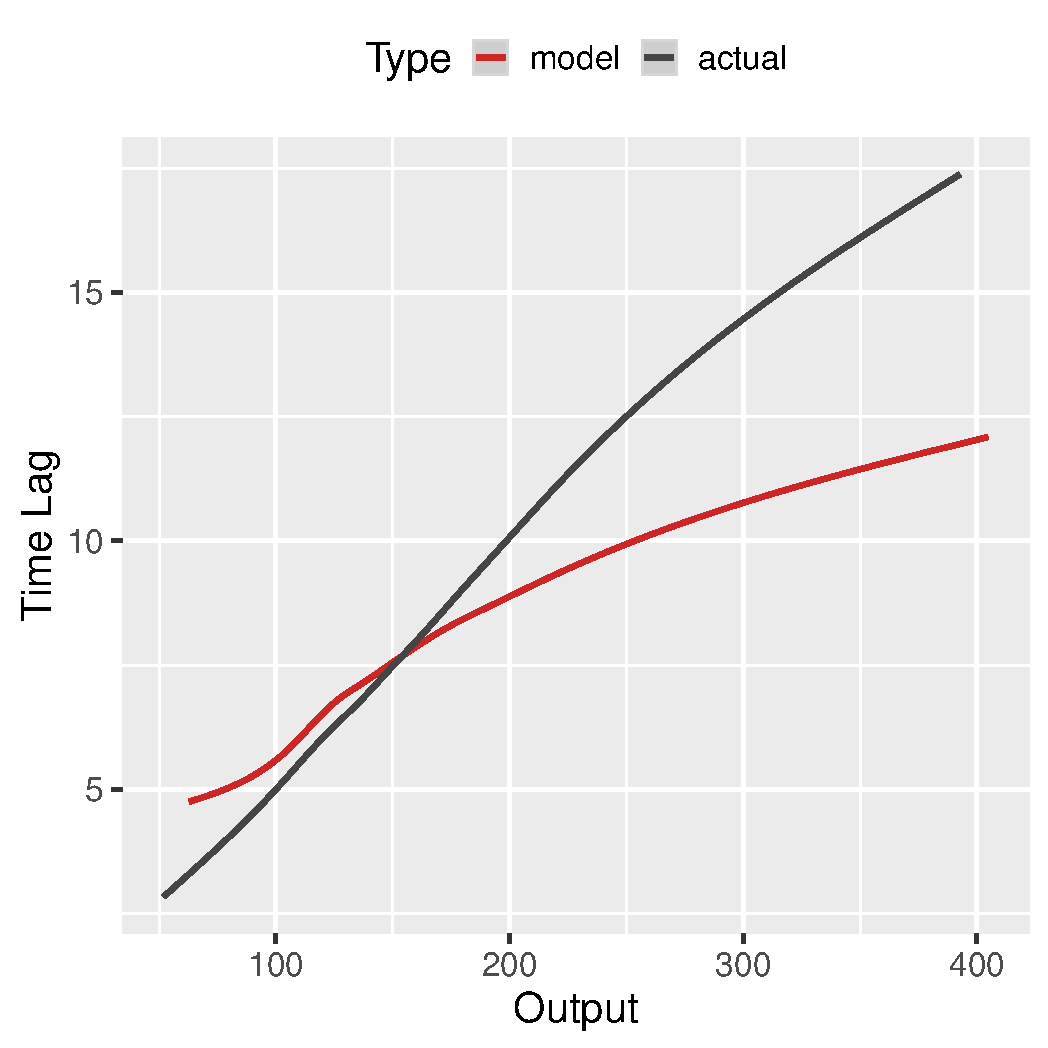
\includegraphics[width=\textwidth]{figures/exp4_predictive_curves}
    \caption{ \textbf{Problem IV}, Output vs Time Lag Relationship} 
    \label{fig:problem4_curves}
  \end{subfigure}
  
  \caption{\textbf{Problem IV}, Results}
\end{figure*}


Table \ref{tab:results_syn} summarises the \XX\ performance on the synthetic and real-world 
problems, respectively compared to the naive baseline (constant time lag) and to the state of the 
art for the real-world solar wind problem. 

The values of the $\sigma_0$ and $C_1$ quantities involved in the stability analysis 
(\cref{sec:stability}) are also reported. As said, $C_1 < 1$ indicates a specialization 
among predictors found by the solution. The comparison of $\sigma_0$ and the RMSE indicates how 
better the learned model is compared to the trivial degenerate solution (uniform $\hat {\bf p}$, 
assigning an equal weight to all $\hat y_i$). Finally, the Pearson correlation between 
$\hat y_t$ and $y_t$ is reported; while its absolute value is less informative than it appears due 
to the auto-correlation of the series, it allows to compare different predictors. 

\begin{table}
  \caption{Performance: \XX  \ / Base Line / \XX  \ Time Lag Prediction}\label{tab:results_syn}
  \centering
  \resizebox{\textwidth}{!}{
    \begin{tabular}{ l l l l l l}
      \hline
      Problem &  M.A.E & R.M.S.E & Pearson Corr. & $\sigma_0$ & $C_1$\\
      \hline
      \textbf{Pb I} & $8.82$ / $21.79$ / $0.021$  & $12.35$ / $28.79$ / $0.26$ & $0.98$ / $0.87$ / -- & $29.8$ & $0.14$\\
      \textbf{Pb II} & $10.15$ / $27.40$ / $0.4$ & $13.70$ / $35.11$ / $0.67$ & $0.95$ / $0.73$ / $0.70$ & $26.83$ & $0.16$\\
      \textbf{Pb III} & $3.17$ / $11.01$ / $0.17$ & $4.63$ / $14.99$ / $0.42$ & $0.98$ / $0.79$ / $0.84$ & $11.84$ & $0.09$\\
      \textbf{Pb IV} & $3.88$ / $12.28$ / $0.34$ & $5.33$ / $15.89$ / $0.64$ & $0.98$ /$0.79$/ $0.81$ & $12.18$ & $0.13$\\
      \textbf{Solar Wind} & $56.35$ / $66.45$ / -- & $74.20$ / $84.53$ / -- & $0.6$ / $0.41$ / -- & $76.46$ & $0.89$\\
      \hline
      \end{tabular}
  }
\end{table}
%\todo{Update $\sigma_0$ and $C_1$ numbers for \XX in \cref{tab:results_syn}}

On the easy Problem I, the model predicts the correct time lag for $97.93\%$ of 
the samples. The higher value of $\sigma_0$ in problems I and II compared to 
the other problems is explained from the higher variance in the generated 
time series $y(t)$. 

On Problem II, the model accurately learns the inverse 
relationship between $\mathbf{x}_t$, $g(\mathbf{x}_t)$ and $y_t$ on average. 
The time lag is overestimated in the regions with low time lag 
(with high velocity), which is blamed on the low sample density in this region, 
due to the data generation process.

Interestingly, Problems III and IV are better handled by \XX, despite a more 
complex dynamic time lag relationship. In both latter cases however, the model 
tends to under-estimate the time lag in the high time lag regions and 
conversely to over-estimate it in the low time lag region. 

\begin{figure}
  \centering
  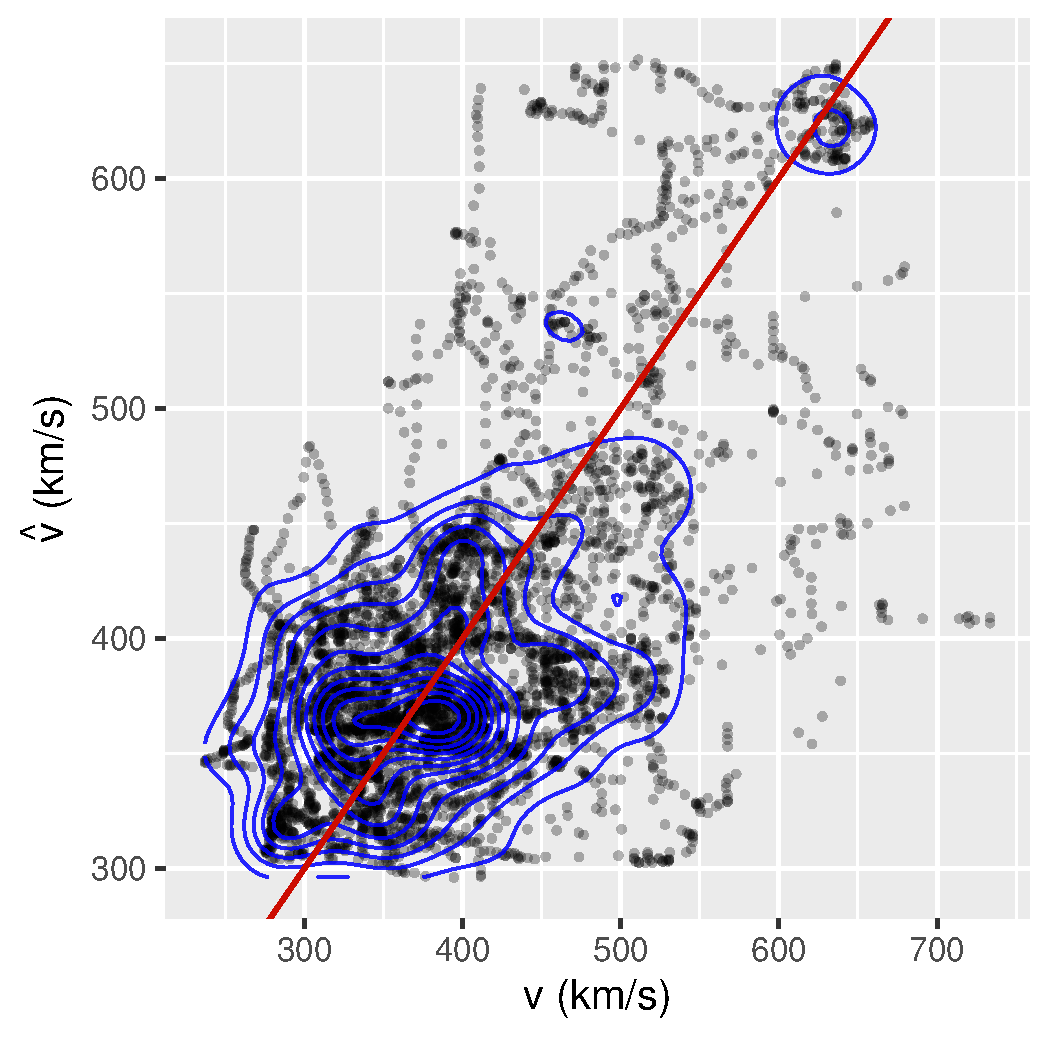
\includegraphics[width=0.4\textwidth]{figures/test_scatter_v}
  \caption{
    Predicted vs Actual Solar Wind Speed, 
    red diagonal represents a perfect prediction and blue lines are contours.} 
  \label{fig:sw_preds}
\end{figure}

Concerning the solar wind problem, \XX\ shows encouraging results on the 
cross-validation experiments as can be seen in \cref{tab:results_syn} and 
visualised in \cref{fig:sw_preds}. The significantly higher difficulty of the 
solar wind forecasting problem is witnessed by the $C_1$ value close to the 
degenerate value of $1$. 
%
In \cref{tab:results_reiss}, we compare the performance of the \XX \ model and the fixed time lag 
baseline with the state of the art from \citet{Reiss_2019}, on the solar wind data from Carrington 
rotation $2077$ (see \cref{table:dtlrsplits}). The \XX \ model gives improvements in predictive 
performance.

\begin{table}
  \caption{
    Performance Comparison on CR $2077$: \XX  \ , 
    Fixed Lag Base Line vs \citet{Reiss_2019}
  }
  \label{tab:results_reiss}
  \centering
  \begin{tabular}{ | l | l l | }
    \hline
    Model &  M.A.E & R.M.S.E \\
    \hline 
    \hline
    WS & $74.09$ & $85.27$ \\
    DCHB & $83.83$ & $103.43$ \\
    WSA & $68.54$ & $82.62$ \\
    Ensemble Median (WS)   & $71.52$ & $83.36$ \\
    Ensemble Median (DCHB) & $78.27$ & $100.04$ \\
    Ensemble Median (WSA)  & $62.24$ & $74.86$ \\
    Persistence (4 days)   & $130.48$ & $161.99$ \\
    Persistence (27 days)  & $66.54$ & $78.86$ \\
    \hline
    Fixed Lag Baseline & $67.33$ & $80.39$ \\
    \hline
    \XX & $60.19$ & $72.64$ \\
  \hline
    \end{tabular}
\end{table}

\begin{figure*}[!htb]
  \centering

  \begin{subfigure}[b]{0.4\textwidth}
    \centering
    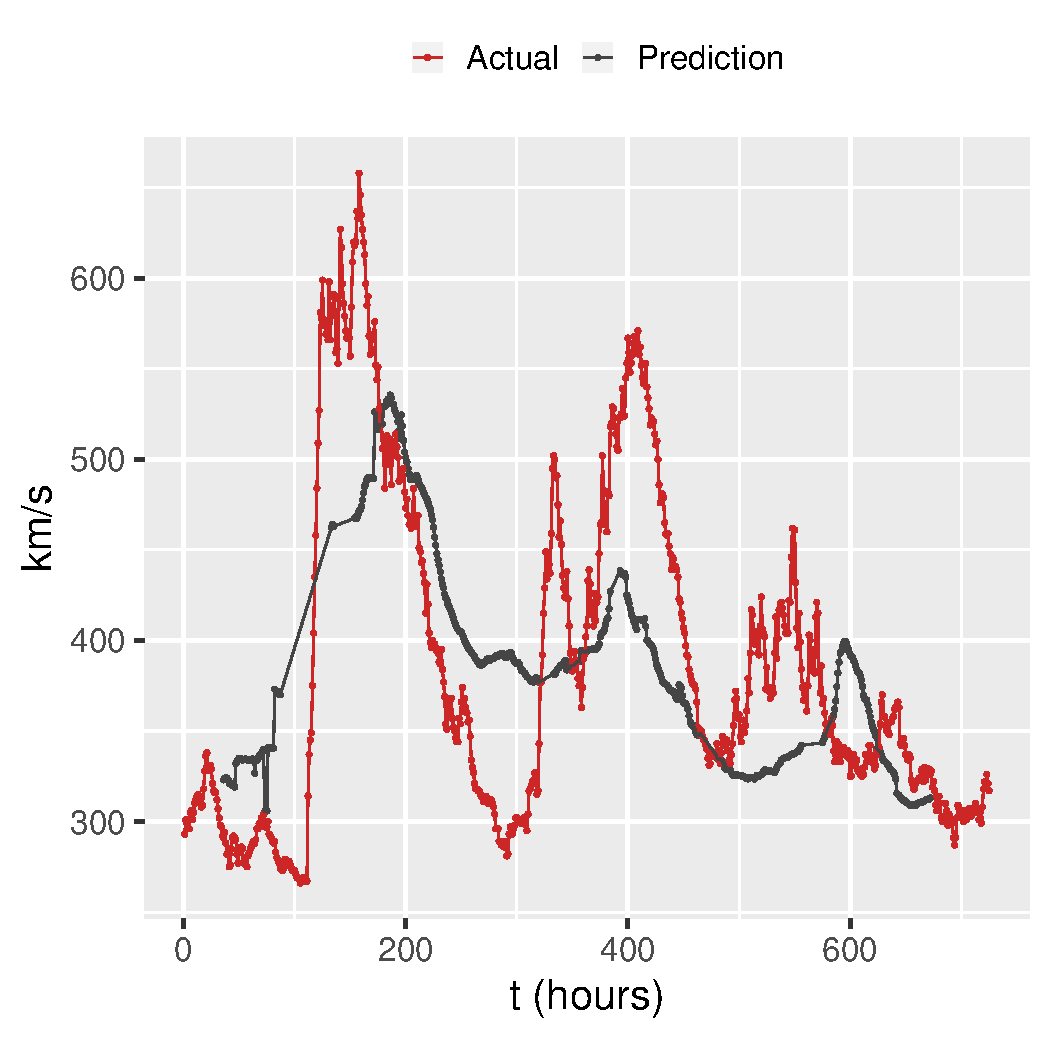
\includegraphics[width=\textwidth]{figures/test_2008-11-20_2008-12-20_ts}
    \caption{Hourly forecasts for the period \\ 2008-11-20 07:00 to 2008-12-17 14:00}
    \label{fig:problemsw_ts1}
  \end{subfigure}
  \hfill
  \begin{subfigure}[b]{0.4\textwidth}
    \centering
    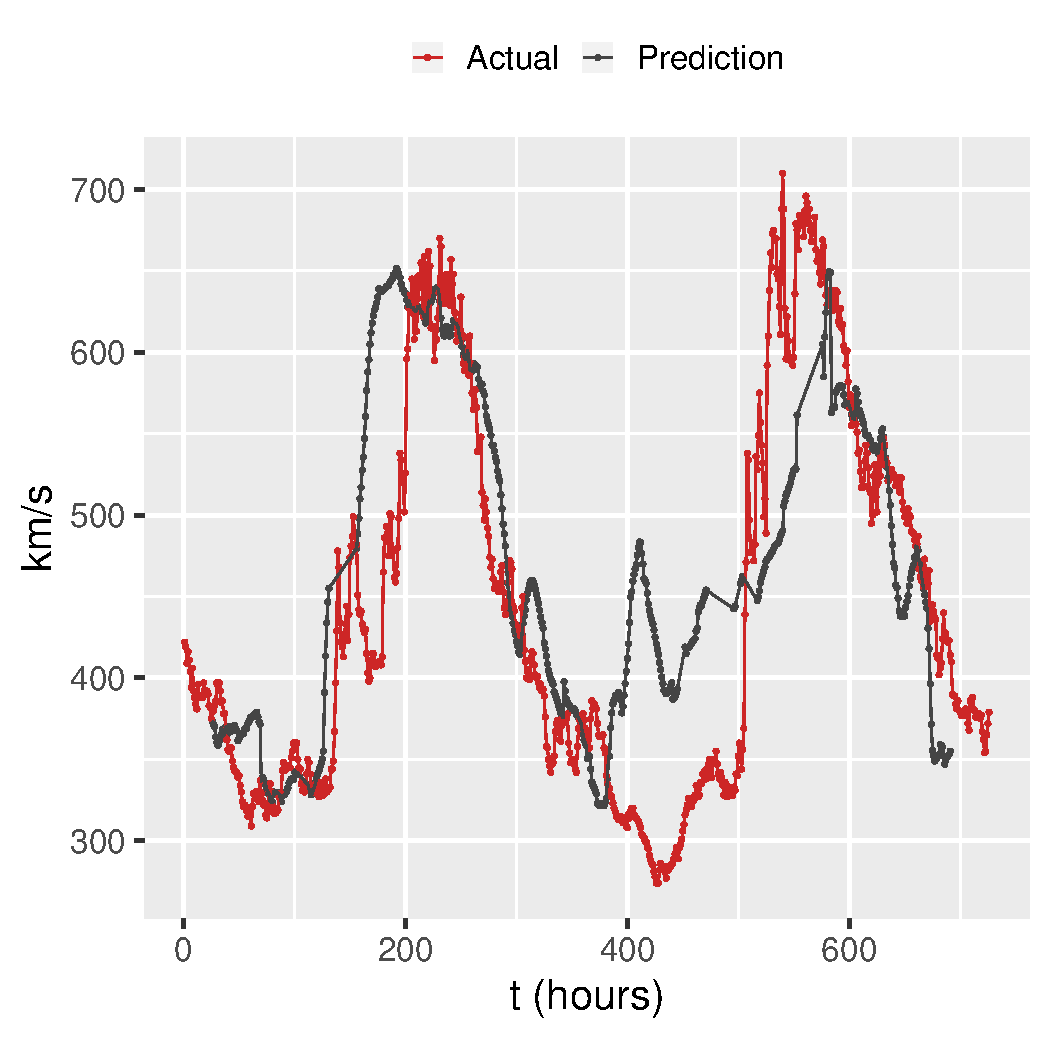
\includegraphics[width=\textwidth]{figures/test_2016-11-16_2016-12-17_ts}
    \caption{ Hourly forecasts for the period \\ 2016-11-16 17:00 to 2016-12-14 01:00}
    \label{fig:problemsw_ts2}
  \end{subfigure}
  
  \caption{\textbf{Solar Wind Prediction}: reconstructed time series predictions}
\end{figure*}

\section{Conclusions}

The contribution of the work is twofold. Firstly, we define a new ML setting, motivated by an 
important scientific and practical problem from the domain of space weather, emphasizing that this 
real-world problem is open for over two decades. This ML setting, called 
Dynamic Time Lag Regression, is concerned with the inference of lagged causal relationships between 
time series. 

Secondly, the proposed \XX\ formalization supports the definition of a nested inference procedure, 
relying on a saddle point optimization process. A closed form analysis of the stability of the 
inferred model under simplifying assumptions has been conducted, yielding a practical alternate 
optimization formulation, implemented in the \XX\ algorithm. The approach demonstrates its merits 
with some proofs of concept on synthetic problems considering time lag models with diverse 
complexity. The application on our motivating real-world problem shows the potential of the 
approach, considering that the \XX\ model involves no domain knowledge in the pre-processing of the 
data or in the sought prediction model. From an applicative perspective, a next step toward 
improving the predictive performances will consist of enriching the data sources and the 
description of the cause series $\mathbf{x}_t$.
%, e.g. augmenting the FTE data set with other solar data sources. Importantly, 

On the methodological side, the longer term research perspective consists of extending the proposed 
nested inference procedure and integrating the model selection step within the inference 
architecture; the challenge is to provide the algorithm with the means of assessing online the 
stability and/or the degeneracy of the learning trajectory. 
%Acknowledgement:
%One of the authors (B.P.) wishes to acknowledge Dr. X. P. Zhao for making the CSSS model 
%available to her and the many discussions.



%\bibliographystyle{plainnat}
%\bibliography{references}
